\documentclass[10.5pt,compsoc,UTF8]{CjC}
\usepackage{CTEX}
\usepackage{graphicx}
\usepackage{footmisc}
\usepackage{subfigure}
\usepackage{url}
\usepackage{multirow}
\usepackage{multicol}
\usepackage[noadjust]{cite}
\usepackage{amsmath,amsthm}
\usepackage{amssymb,amsfonts}
%\usepackage{booktabs}
\usepackage{color}
\usepackage{ccaption}
\usepackage{makecell}
\usepackage{booktabs}
\usepackage{float}
\usepackage{fancyhdr}
\usepackage{caption}
\usepackage{xcolor,stfloats}
\usepackage{comment}
\setcounter{page}{1}
\graphicspath{{figures/}}
\usepackage{cuted}
\usepackage{captionhack}
\usepackage{epstopdf}
\usepackage{gbt7714}
\usepackage{stfloats}
\usepackage{amsmath}
\usepackage{arydshln}

%===============================%

%=======设置奇偶页页眉=======%
\headevenname{\mbox{\quad} \hfill  \mbox{\zihao{-5}{计\quad \quad 算\quad \quad 机\quad \quad 学\quad \quad 报} \hspace {50mm} \mbox{2023 年}}}%
\headoddname{? 期 \hfill
方维等:深度脉冲神经网络梯度替代学习算法研究综述}
%=======设置奇偶页页眉=======%

\renewcommand{\thefootnote}{\fnsymbol{footnote}}
\setcounter{footnote}{0}
\renewcommand\footnotelayout{\zihao{5-}}
\newtheoremstyle{mystyle}{0pt}{0pt}{\normalfont}{1em}{\bf}{}{1em}{}
\theoremstyle{mystyle}
\renewcommand\figurename{figure~}
\renewcommand{\thesubfigure}{(\alph{subfigure})}
\newcommand{\upcite}[1]{\textsuperscript{\cite{#1}}}
\renewcommand{\labelenumi}{(\arabic{enumi})}
\newcommand{\tabincell}[2]{\begin{tabular}{@{}#1@{}}#2\end{tabular}}
\newcommand{\abc}{\color{white}\vrule width 2pt}
\renewcommand{\bibsection}{}
\makeatletter
\renewcommand{\@biblabel}[1]{[#1]\hfill}
\makeatother
\setlength\parindent{2em}

\pagestyle{CjCheadings}
\setmainfont{Times New Roman}

%===========================================================%
\begin{document}

\hyphenpenalty=50000
\makeatletter
\newcommand\mysmall{\@setfontsize\mysmall{7}{9.5}}
\newenvironment{tablehere}
  {\def\@captype{table}}

\let\temp\footnote
\renewcommand \footnote[1]{\temp{\zihao{-5}#1}}

%=======设置首页页眉=======%
\thispagestyle{empty}%
\begin{table*}[!t]
\vspace {-13mm}
\onecolumn
\noindent\begin{tabular}{p{168mm}}
\zihao{5-}
第??卷\quad 第?期 \hfill 计\quad 算\quad 机\quad 学\quad 报\hfill Vol. ??  No. ?\\
\zihao{5-}
20??年?月 \hfill CHINESE JOURNAL OF COMPUTERS \hfill ???. 20??\\
\hline\\[-5.5mm]
\hline\end{tabular}\end{table*}
%=======设置首页页眉=======%

%中文标题、作者与注脚
{
\centering
\vspace {11mm}
{\zihao{2} \heiti 深度脉冲神经网络梯度替代学习算法研究综述}

\vskip 5mm

{\zihao{3}\fangsong 方维$^{1)}$\quad 朱耀宇$^{2)}$\quad 黄梓涵$^{3)}$\quad 姚满$^{4)}$\quad 余肇飞$^{6),3)}$\quad 田永鸿$^{1),3),5)}$}

\let\thefootnote\relax\footnote{\noindent \zihao{6}\songti 收稿日期:\quad \quad -\quad -\quad ;最终修改稿收到日期:\quad \quad -\quad -\quad . 本课题得到国家自然科学基金(No.62425101, 62332002, 62027804, 62088102)资助.\textsf{方维},男,博士,助理研究员,主要研究领域为脉冲深度学习.E-mail: fwei@pku.edu.cn.\textsf{朱耀宇},男,博士,特任研究助理,主要研究领域为类脑计算.E-mail: zhuyaoyu@ict.ac.cn. \textsf{黄梓涵},男,博士研究生,主要研究领域为神经形态计算.E-mail: hzh@stu.pku.edu.cn. \textsf{姚满},男,博士,特任研究助理,主要研究领域为神经形态计算.E-mail: man.yao@ia.ac.cn. \textsf{余肇飞},男,博士,助理教授,主要研究领域为计算机视觉、神经形态计算和计算神经科学. E-mail: yuzf12@pku.edu.cn.\textsf{田永鸿},博士,教授,中国计算机学会(CCF)高级会员,主要研究领域为视频大数据分析处理、机器学习、类脑计算. E-mail: yhtian@pku.edu.cn. 第1作者手机号码: 13041160166, E-mail: fangwei123456g@gmail.com.}

\vspace {1mm}

\zihao{6}{$^{1)}$(北京大学深圳研究生院信息工程学院,深圳,518055)}

\zihao{6}{$^{2)}$(中国科学院计算技术研究所,北京,100190)}

\zihao{6}{$^{3)}$(北京大学计算机学院,北京,100871)}

\zihao{6}{$^{4)}$(中国科学院自动化研究所,北京,100190)}

\zihao{6}{$^{5)}$(鹏城实验室,深圳,518000)}

\zihao{6}{$^{6)}$(北京大学人工智能研究院,北京,100871)}

}%中文标题、作者与注脚

\vskip 5mm

\zihao{5-}{
\setlength{\baselineskip}{16pt}\selectfont{
\noindent {\heiti 摘\quad 要\quad }
被誉为第三代神经网络模型的脉冲神经网络(Spiking Neural Network, SNN)具有二值通信、稀疏激活、事件驱动、超低功耗的特性,但也因复杂的时域动态、离散不可导的脉冲发放过程难以训练.近年来以梯度替代法和人工神经网络(Artificial Neural Network, ANN)转换SNN方法为代表的深度学习方法被提出,大幅度改善SNN性能,形成了脉冲深度学习这一全新领域.本文围绕梯度替代法的研究进展,对其中的基础学习算法、ANN辅助训练算法、神经元和突触改进、网络结构改进、正则化方法、事件驱动学习算法、在线学习算法以及训练加速方法进行系统性地回顾和综述,讨论了各类方法的优缺点,并展望了未来可能取得突破的研究方向.
\quad}}

\vspace {5mm}

\zihao{5-}{\noindent
{\heiti 关键词 \quad }{脉冲神经网络;梯度替代法;类脑计算;神经形态计算;脉冲深度学习}
}\par\noindent
\zihao{5-}{\heiti 中图法分类号\quad } TP\rm{\quad \quad \quad     }
{\heiti DOI号:\quad } *投稿时不提供DOI号

\vskip 5mm

\begin{center}
\zihao{3}{\heiti Review of surrogate learning methods in deep spiking neural networks}{Review of surrogate learning methods in deep spiking neural networks}\\
\vspace {5mm}
\zihao{5}{ Wei Fang$^{1)}$\quad Yaoyu Zhu$^{2)}$\quad Zihan Huang$^{3)}$\quad Man Yao$^{4)}$\quad Zhaofei Yu$^{6),3)}$\quad Yonghong Tian$^{1),3),5)}$}\\
\vspace {1mm}
\zihao{6}{{$^{1)}$School of Electronic and Computer Engineering, Shenzhen Graduate School, Peking University, Shenzhen, 518055}}

\zihao{6}{{$^{2)}$(Institute of Computing Technology, Chinese Academy of Sciences, Beijing 100190)}}

\zihao{6}{{$^{3)}$(School of Computer Science, Peking University, Beijing, 100871)}}

\zihao{6}{{$^{4)}$(Institute of Automation, Chinese Academy of Sciences, Beijing, 100190)}}

\zihao{6}{{$^{5)}$(Peng Cheng Laboratory, Shenzhen, 518000)}}

\zihao{6}{{$^{6)}$(Institute for Artificial Intelligence, Peking University, Beijing, 100871)}}
\end{center}

\zihao{5}{{\noindent\bf Abstract}\quad
\zihao{5}{\noindent Spiking Neural Networks (SNNs) are regarded as the third generation of neural network models with binary communication, sparse activation, event-driven, and extremely power-efficient characteristics. However, the training of SNNs is difficult because of their complex temporal dynamics and non-differentiable firing mechanisms. Recently, deep learning methods, including the surrogate gradient methods and the Artificial Neural Networks (ANN) to SNN conversion methods, have proposed and promoted the performance of SNNs greatly, which develops the Spiking Deep Learning area. This article focuses on the advances of surrogate gradient methods and reviews the basic learning methods, ANN-auxiliary training methods, neuron and synapse model modifications, network structure designs, normalization methods, event-driven learning methods, and training acceleration methods systemically. Finally, the potential breakthrough research topics are prospected.
\par}}

\vspace {5mm}

\zihao{5}{
{\noindent\bf Keywords}\quad Spiking Neural Networks, Surrogate Gradient Methods, Brain-inspired Computing, Neuromorphic Computing, Spiking Deep Learning
\par}

\zihao{5}
\vskip 1mm
\begin{multicols}{1}

\section{引言}
人工智能在最近十几年取得了跳跃式的发展\upcite{deep-learning-nature},在图像分类\upcite{he2015delving, szegedy2015going, he2016deep, dosovitskiy2020image}、目标检测和跟踪\upcite{girshick2014rich, redmon2016you}、语音识别\upcite{graves2013speech, graves2013hybrid}、机器翻译\upcite{sutskever2014sequence, bahdanau2014neural, sennrich2015neural}、游戏对战\upcite{mnih2015human, silver2017mastering}、聊天机器人\upcite{NEURIPS2020_1457c0d6, zeng2021pangualphalargescaleautoregressivepretrained, openai2024gpt4technicalreport}、图像生成\upcite{NIPS2014_5ca3e9b1, DBLP:journals/corr/RadfordMC15, Rombach_2022_CVPR}等领域取得了突破性进展,引领了新一轮的经济发展和产业变革.在人工智能的发展过程中,神经科学提供的视野和灵感起到了重要作用\upcite{hassabis2017neuroscience, Zador2023},最典型的例子莫过于神经网络,其起源于神经科学,并在人工智能领域作为最主要的计算模型.

第一代神经网络又称为感知机(Perceptron)\upcite{rosenblatt1958perceptron},接收多个输入并输出布尔值,可以通过训练解决线性分类问题,引发了第一次神经网络热潮.感知机不能处理非线性的异或(XOR)问题,且训练算法只能用于单层网络,这些缺点使得对神经网络的关注逐渐衰退.
第二代神经网络人工神经网络(Artificial Neural Network, ANN)不再输出布尔值,而是改用Sigmoid等非线性激活输出,结合反向传播算法\upcite{rumelhart1986learning}实现多层网络的构建和训练,解决了异或分类问题,引发了第二次神经网络热潮.但受限于芯片行业的发展,90年代的算力无法支撑大规模神经网络的训练,而小规模神经网络在计算代价、任务性能、可解释性等方面相较于支持向量机\upcite{cortes1995support}等当时人工智能领域的主流方法并不占优,因而对神经网络的研究又逐渐陷入第二次低谷.
脉冲神经网络(Spiking Neural Network, SNN)被誉为第三代神经网络模型\upcite{maass1997networks},与生物神经元的机制更为相似,拥有积分发放、阈值触发、稀疏激活、脉冲通信的特性.SNN凭借极高的生物可解释性,已经被计算神经科学领域广泛使用\upcite{gewaltig2007nest, spaun, Stimberg2019},用于解释和探究生物神经系统的运行原理.由于复杂的时域动态、离散不可导的脉冲发放过程,训练SNN比ANN更为困难,因而SNN在任务性能为主要导向的人工智能领域的地位一度较为边缘.

神经形态计算(Neuromorphic Computing)\upcite{mead1990neuromorphic, roy2019towards}的蓬勃发展为SNN提供了新的机遇.神经形态计算是一种全新的计算范式,旨在借鉴和模仿大脑的运行机理,实现超越传统冯诺依曼架构(Von Neumann Architecture)的全新软件算法和硬件设备,代表性成果包括动态视觉传感器(Dynamic Vision Sensor, DVS)\upcite{lichtsteiner2008128}、视达(Vidar)\upcite{dong2017spike}等神经形态视觉传感器和IBM True North\upcite{merolla2014million}、Intel Loihi\upcite{loihi}、浙江大学达尔文(Darwin)\upcite{ma2017darwin}、清华大学天机芯(Tianjic)\upcite{pei2019towards}等神经形态计算芯片.SNN被视作神经形态计算领域的主要计算模型,有望结合神经形态视觉传感器和计算芯片,充分利用脉冲计算的二值量化、稀疏激活特性,实现感算一体、事件驱动的超低功耗边缘智能(Edge AI)系统\upcite{roy2019towards},但这一设想受限于SNN高性能学习算法的缓慢发展,一度难以实现.

2006年Hinton等\upcite{10.1162/neco.2006.18.7.1527}使用神经网络在MNIST数据集\upcite{MNIST}上击败了基于径向基函数内核(Radial Basis Function Kernel)的支持向量机,以深度学习(Deep Learning)之名拉开了神经网络复兴的序幕\upcite{Goodfellow-et-al-2016}.
2012年Alex等\upcite{NIPS2012_c399862d}构建了大规模深度卷积神经网络AlexNet并借助图形处理单元(Graphics Processing Unit, GPU)的强大并行计算能力训练,在ImageNet大规模图像识别挑战赛\upcite{russakovsky2015imagenet}上取得第一,相较于第二名有着10\%正确率的断崖式性能领先,引发了第三次神经网络热潮.
深度学习方法以革命般摧枯拉朽的力量将人工智能的各个领域重塑,%甚至蔓延到更广泛的其他学科,形成人工智能驱动的科学研究(AI for Science)\upcite{Jumper2021, doi:10.1126/science.adg7492, Bi2023, Wang2023}这一全新研究范式.
在这一过程中,以梯度替代法(Surrogate Learning Method)\upcite{neftci2019surrogate}和ANN转换SNN方法(ANN to SNN Conversion, ANN2SNN)\upcite{cao2015spiking}为代表的两大类深度学习方法被应用于SNN的训练,大幅提升SNN的任务性能至早期ANN的水平\upcite{TAVANAEI201947},形成了脉冲深度学习(Spiking Deep Learning)这一研究领域.梯度替代法直接训练深度SNN,训练开销大,但获得的SNN仿真步数少、延迟低,不局限于频率编码且能够用于神经形态数据分类等时域任务;ANN2SNN方法则是将已有的ANN转换为SNN,避免训练开销,转换速度快、任务精度高,但通常基于频率编码,仿真步数多、延迟高且不能用于时域任务.本文聚焦直接训练方法,对基于梯度替代法的深度SNN学习算法进行系统性介绍和总结.

\section{深度脉冲神经网络的基本组分和评测基准}
深度SNN通常由多个突触层和脉冲神经元层堆叠而成.
SNN的突触层,与ANN中的基本一致,主要包括卷积层、池化层、全连接层等.批量标准化(Batch Normalization, BN)\upcite{ioffe2015batch}和层标准化(Layer Normalization, LN)\upcite{ba2016layer}等正则化层也经常被使用.
SNN的脉冲神经元是其区别于ANN的显著标志,与生物神经系统中的神经元行为更为相似.生物神经元接收其他神经元通过树突(Dendrite)传递来的输入电信号,累计为自身的膜电位(Membrane Potential),当膜电位超过阈值(Threshold)电位时,神经元会将累计的电荷在极短的时间内(约为1--2毫秒)一次性释放,形成脉冲(Spike)并通过轴突(Axon)传递到其他神经元.
神经元释放脉冲后,膜电位会瞬间降低,这一过程称之为放电后的重置(Reset).

计算神经科学中构建的脉冲神经元模型,对生物神经元进行了精细建模,通常使用一个或多个微分方程去描述其神经动态.例如,使用最为广泛的泄露积分发放(Leaky Integrate-and-Fire, LIF)神经元的阈下神经动态为:
\begin{eqnarray}
	\tau_{m} \frac{\mathrm{d}V(t)}{\mathrm{d}t} = -(V(t) - V_{rest}) + X(t),
	\label{eq, continuous LIF neuronal charge}
\end{eqnarray}
其中$\tau_{m}$是膜时间常数,$V(t)$是膜电位,$V_{rest}$是静息电位,$X(t)$是输入电流.如果膜电位$V(t)$超过了阈值,则释放脉冲,使用Heaviside阶跃函数$\Theta(x)$描述这一过程:
\begin{eqnarray}
	S(t) = \Theta(V(t) - V_{th}),
	\label{eq, continuous neuronal fire}
\end{eqnarray}
其中$x \ge 0$时$\Theta(x) = 1$,$x < 0$时$\Theta(x) = 0$.
当神经元释放脉冲后,膜电位瞬间重置到$V_{reset}$,这一重置过程可以描述为:
\begin{eqnarray}
	\lim_{\Delta t \rightarrow 0^{+}} V(t + \Delta t) = V_{reset}. \label{eq, continuous neuronal reset}
\end{eqnarray}
诸如Izhikevich模型\upcite{izhikevich2003simple}等更为精细的脉冲神经元模型通常需要更多数量的微分方程去描述,计算代价较高,因而在深度SNN中较少使用.
对脉冲神经元进行仿真时,通用做法是将连续时间微分方程转换为离散时间差分方程.Fang等\upcite{fang2021incorporating, doi:10.1126/sciadv.adi1480}使用充电、放电、重置三个方程来构建通用离散时间脉冲神经元模型:
\begin{align}
	H[t] &= f(V[t-1], X[t]), \label{eq, discrete neuronal charge}\\
	S[t] &= \Theta(H[t] - V_{th}), \label{eq, discrete neuronal fire}\\
	V[t] &= \begin{cases}
		H[t] \cdot (1 - S[t]) + V_{reset} \cdot S[t], \text{硬重置}\\
		H[t] - V_{th} \cdot S[t], \text{软重置}
	\end{cases}. \label{eq, discrete neuronal reset}
\end{align}
其中$H[t]$表示充电后、重置前的膜电位,$X[t]$表示输入电流,$V_{th}$表示阈值,$S[t]$表示释放的脉冲,$V[t]$表示重置后的膜电位,$V_{reset}$表示重置电压.
公式(\ref{eq, discrete neuronal charge})表示神经元的充电方程,$f$因神经元而异,例如对于LIF神经元而言,参考其微分方程(\ref{eq, continuous LIF neuronal charge})式,可以得到充电的差分方程为:
\begin{eqnarray}
	H[t] = V[t-1] + \frac{1}{\tau_{m}}(X[t]-(V[t-1] - V_{rest})).
	\label{eq, discrete LIF neuronal charge}
\end{eqnarray}
公式(\ref{eq, discrete neuronal fire})为放电方程,使用Heaviside阶跃函数来比较膜电位和阈值,并生成二值脉冲.
公式(\ref{eq, discrete neuronal reset})为重置方程,目前在脉冲深度学习领域主要存在两种重置方法,分别为硬重置(Hard Reset)和软重置(Soft Reset).硬重置在释放脉冲后,将膜电位直接设置为$V_{reset}$,研究者们发现其用于梯度替代法训练的深度SNN性能较好\upcite{ledinauskas2020training}.软重置则是在神经元释放脉冲后,将膜电位减少$V_{th}$,使用这种重置方式的积分发放(Integrate-and-Fire, IF)神经元在理论上拟合ReLU函数的误差更小\upcite{Bodo2017Conversion},因而在ANN2SNN中普遍使用.

脉冲深度学习蓬勃发展,大量研究结果不断涌现,其中静态图像数据集和神经形态数据集分类任务是最频繁使用的性能评测基准.图像数据集的“静态”是相较于动态的神经形态数据而言,因图像通常不包括时域信息.常用的静态图像数据集包括MNIST\upcite{MNIST}、Fashion-MNIST\upcite{FMNIST}、CIFAR\upcite{CIFAR10}和ImageNet\upcite{russakovsky2015imagenet}数据集,数据集规模和分类难度依次递增.神经形态数据集是从神经形态视觉传感器直接收集或软件仿真算法将静态图片转换而得到的事件集合,其中每个事件通常以异步的地址事件协议(Address Event Representation, AER)来表示为$(x_{i},y_{i},t_{i},p_{i})$,其中$i$是事件索引,$(x_{i},y_{i})$是事件的横纵坐标,$t_{i}$是事件的时间戳,$p_{i} \in \{-1, 1\}$是事件的极性.神经形态数据集中的事件稀疏但数量众多,一个样本通常包含百万个事件,难以被神经网络直接处理,因而需要通过切片积分等下采样方式转换成帧数据后才能使用\upcite{wu2018STBP, fang2021incorporating, doi:10.1126/sciadv.adi1480}.常用的神经形态数据集包括N-MNIST\upcite{10.3389/fnins.2015.00437}、CIFAR10-DVS\upcite{10.3389/fnins.2017.00309}、DVS Gesture\upcite{amir2017low}、ASL-DVS\upcite{Bi_2019_ICCV} N-Caltech101\upcite{10.3389/fnins.2015.00437}、ES-ImageNet\upcite{10.3389/fnins.2021.726582}、Spiking Heidelberg Digits (SHD)\upcite{shd}等.神经形态数据集常用于评估SNN的时域信息处理能力. 但Laxmi等\upcite{10.3389/fnins.2021.608567}等指出多数神经形态数据集的时域信息较少,因而对于网络的长期依赖学习能力评估,序列(Sequential)图像分类更为常用\upcite{yin2021accurate, fang2023parallel}.在序列图像分类任务中,图像会被从左到右逐列输入,网络在同一个时刻只能看到一列图像,因而最终的分类结果能够体现网络的记忆能力.

\section{深度脉冲神经网络的梯度替代训练算法}
%SNN具有稀疏激活、脉冲通信、事件驱动的特性,在神经形态计算芯片上运行时拥有高达数千倍于传统芯片的能耗优势\upcite{merolla2014million, loihi, roy2019towards},
由于高性能学习算法的缺失,SNN一度只能解决MNIST分类这种玩具级别的任务,不具备处理现实世界问题的能力.
近年来随着脉冲深度学习方法的相继提出,SNN的性能大幅度提升至实用水平,研究者们甚至成功构建出基于脉冲计算的超低功耗边缘智能设备\upcite{pei2019towards, Yao2024, Yang2024}.本章将对脉冲深度学习方法中的梯度替代法这一大类算法进行详细介绍,全面梳理现有研究成果和最新进展.


\subsection{基础学习算法}% 例如slayer、stbp
SNN不能直接使用梯度下降和反向传播训练算法的原因在于,脉冲发放过程,即(\ref{eq, discrete neuronal fire})式使用的Heaviside阶跃函数$\Theta(x)$,其梯度为冲击函数$\delta(x)$:
\begin{align}
	\Theta'(x) = \delta(x) = \begin{cases}
		+\infty, x = 0\\
		0, x \ne 0,
	\end{cases}.
\end{align}
在反向传播中使用$\delta(x)$会破坏正常的梯度传播,使得网络无法训练.Wu等\upcite{wu2018STBP}、Zenke等\upcite{10.1162/neco_a_01086}、Shrestha等\upcite{shrestha2018slayer}在2018年分别独立地提出了梯度替代方法,成为目前直接训练深度SNN算法的基石.梯度替代法在前向传播时使用Heaviside阶跃函数$\Theta(x)$生成二值脉冲,而在反向传播时重定义$\Theta'(x)$为替代函数$\sigma(x)$的导数$\sigma'(x)$.具体而言,(\ref{eq, discrete neuronal fire})式仍然用于前向传播,而其反向传播的按照$\frac{\partial S[t]}{\partial (H[t] - V_{th})} = \sigma'(H[t] - V_{th})$.
替代函数$\sigma(x)$通常是连续、光滑的函数,拥有数值正常的梯度,可以视作$\Theta(x)$的近似.常用的替代函数包括Rectangular\upcite{wu2018STBP}、SuperSpike\upcite{10.1162/neco_a_01086}、ArcTan\upcite{fang2021incorporating}、Sigmoid等.尚无理论明确哪种替代函数是最优的,Zenke等\upcite{Zenke2020.06.29.176925}通过网格搜索的实验性结论表明,不同的替代函数能达到的最优性能相同,但对超参数的敏感度存在很大差异,因而替代函数的选择对网络训练较为关键.Li等\upcite{li2021differentiable}使用数值梯度来辅助替代函数形状参数的选取,取得了比常规替代函数更好的训练结果.

\subsection{ANN辅助训练}
% 由于SNN神经元间采用可以仅通过加法实现的脉冲通信方式,再加上脉冲的稀疏特性使其相对于需要大量乘法实现的ANN具有极高的能耗优势.然而由于脉冲发放机制的存在,脉冲神经元的梯度无法直接应用于梯度下降,仅使用代替梯度进行训练,得到的SNN网络大多性能不如ANN网络,且在训练过程中较容易遇到梯度爆炸或者梯度消失的问题,导致在训练深层的SNN时难以收敛.(考虑删除)
为了充分利用ANN的性能优势与SNN的能耗优势,一些研究者通过ANN辅助训练来获得高性能的SNN,主要分为两类方法:基于共享权重训练的方法和基于蒸馏的SNN训练.


\begin{figure}[H]
	\centerline{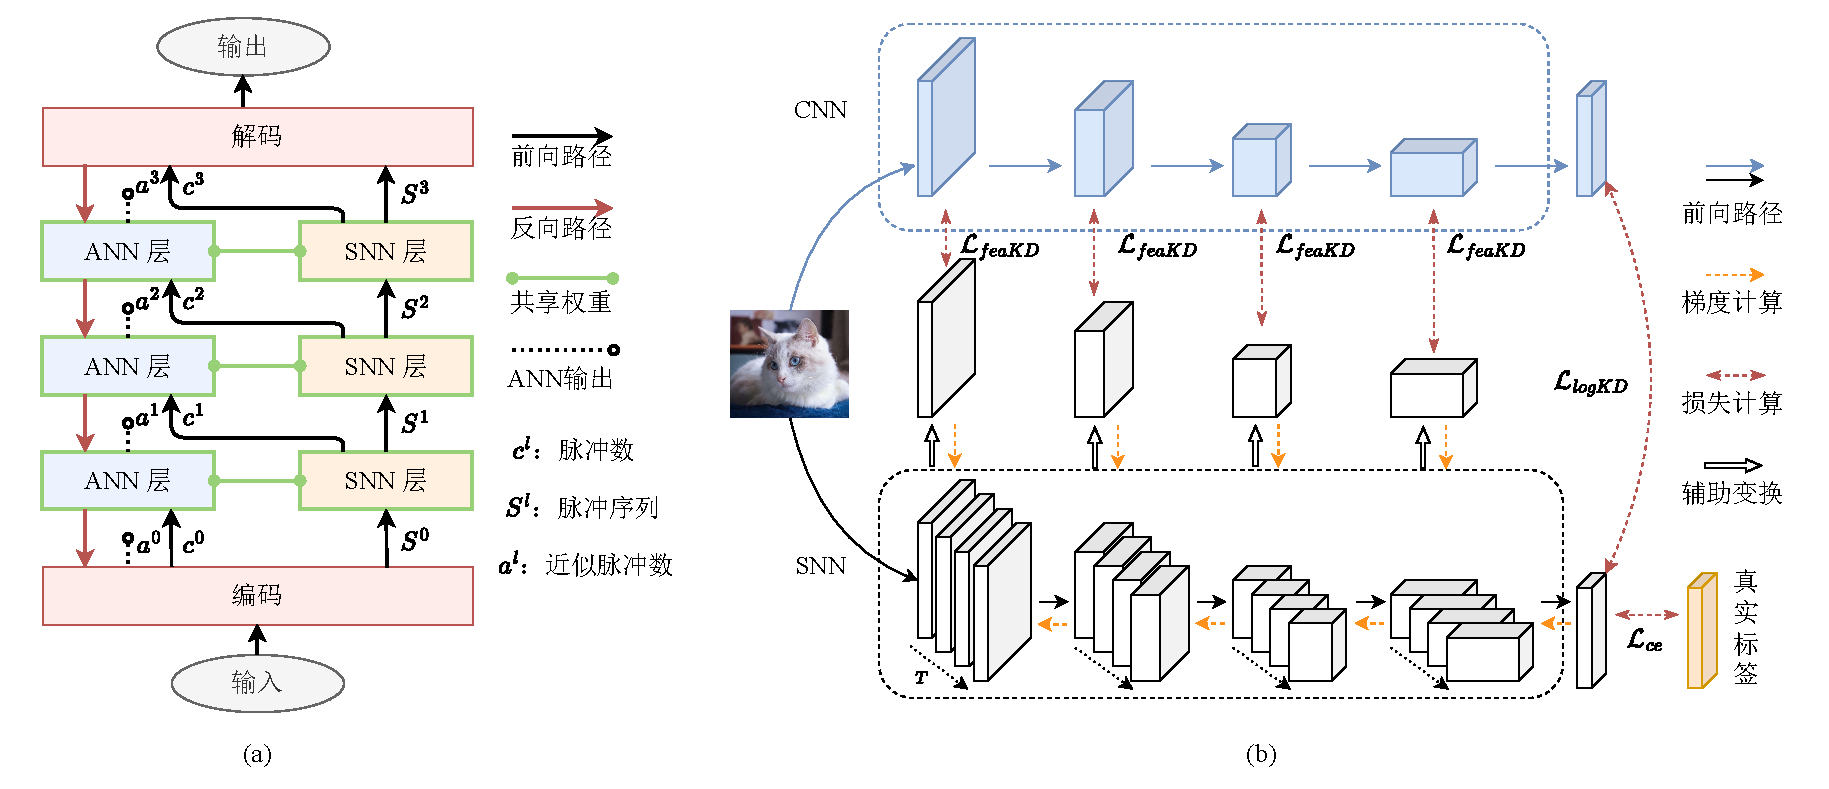
\includegraphics[width=0.5\textwidth,trim=0 0 0 0,clip]{./data/assist.drawio.pdf}}
	{\zihao{5}图X\quad 两类ANN辅助训练方法. (a)共享权重方法. (b)蒸馏方法}
	\label{fig:assist}
\end{figure}

基于共享权重的训练中,Wu等\upcite{wu2021tandem}和Kheradpisheh等\upcite{kheradpisheh2022spiking}设计了共享相同权重的SNN网络和ANN网络,以SNN的输出在时间上的累计近似ANN的激活值,通过在ANN的反向传播来更新共享权重.具体而言,Wu等\upcite{wu2021tandem}提出一种串联学习框架,该框架包括一个SNN和一个通过权重共享耦合的ANN.图\ref{fig:assist}(a)展示了该串联学习框架,在前向传播时SNN结构利用前一层输出的脉冲序列$S^{l-1}$计算当前层的输出脉冲序列$S^l$和脉冲数$c^l=\sum_{t=0}^{T-1} S^l[t]$,而ANN则利用前一层的脉冲数$c^{l-1}$计算当前层的激活值$a^l$来近似脉冲数.在反向传播时,使用ANN的激活值$a^l$的梯度代替脉冲数$c^l$的梯度,通过ANN的反向传播计算前一层激活值和权重的梯度:
\begin{align}
	&\frac{\partial \mathcal{L}}{\partial a^{l-1}} \approx \frac{\partial \mathcal{L}}{\partial c^{l-1}} = \frac{\partial \mathcal{L}}{\partial a^l} \cdot \frac{\partial a^l}{\partial c^{l-1}},\\
	&\frac{\partial \mathcal{L}}{\partial W^{l-1}} =  \frac{\partial \mathcal{L}}{\partial a^{l-1}} \cdot \frac{\partial a^{l-1}}{\partial W^{l-1}},
\end{align}
其中$\mathcal{L}$是模型的损失,$W^{l-1}$是第$l-1$层的权重.该方法在ANN中计算SNN输出的误差,使用ANN的梯度代替SNN的梯度更新权重,避开了脉冲释放过程不可导的问题,且不需要在每个时间步都进行复杂的梯度计算.

Kheradpisheh等\upcite{kheradpisheh2022spiking}设计了一对由IF神经元组成的SNN网络和由ReLU激活函数组成的ANN网络,两个网络共享权重.该网络利用IF神经元输出的频率来近似ReLU神经元的输出,用SNN的输出近似ANN的输出.
不同于Wu等\upcite{wu2021tandem}在前向传播时将SNN脉冲数作为ANN层的输入,Kheradpisheh等\upcite{kheradpisheh2022spiking}在前向传播时分别运行SNN和ANN,在反向传播时,该方法不是直接计算ANN的真实梯度,而是将ANN输出替换为SNN输出,从而在ANN中计算SNN的近似梯度:
\begin{align}
	&\mathcal{L}=-\sum_k{Y_{k}\mathrm{ln}(O_k^A)}\approx-\sum_k{Y_{k}\mathrm{ln}(O_k^S)},\\
	&\frac{\partial \mathcal{L}}{\partial W^l_{ji}}=\sum_k{\frac{\partial \mathcal{L}}{\partial O^A_{k}}\sum_d{\frac{\partial O^A_k}{\partial y^L_d}\frac{\partial y^L_d}{\partial W^l_{ij}}}}\approx \sum_k{\frac{\partial \mathcal{L}}{\partial O^S_{k}}\sum_d{\frac{\partial O^S_k}{\partial y^L_d}\frac{\partial y^L_d}{\partial W^l_{ij}}}},
\end{align}
其中,$\mathcal{L}$是网络的损失函数,$Y_k$是第$k$类的目标值,如果样本为第$k$类,则$Y_k$为1,否则为0;$y^L_{d}$是代理ANN网络最后一层第$d$个神经元的输出,$O^A_k$、$O^S_k$是代理ANN网络和SNN网络的在第$k$个类别的输出,$W^l_{ij}$是第$l$层的权重.该方法用SNN的输出$O^S_k$替换ANN的输出$O^A_k$,从而在ANN模型中反向传播计算SNN模型的误差.共享权重类方法直接避开了SNN计算代价高、训练耗时长的反向传播流程,但由于ANN和SNN本身的差异,共享权重和不精确的梯度会导致训练出的SNN性能较其耦合的ANN有较大程度下降.

基于蒸馏的SNN训练中,Xu等\upcite{xu2023constructing}和Qiu等\upcite{qiu2024self}利用知识蒸馏方法,SNN模型作为学生从教师ANN模型中学习,该方法可以在很短的时间步长上有效地构建深层SNN网络. Xu等\upcite{xu2023constructing}提出了基于响应的知识蒸馏和基于特征提取的知识蒸馏两种方法.基于响应的知识蒸馏只从教师ANN模型的最后一层的输出中提取知识,其损失函数包含SNN输出$Q_s$与真实标签$y_{true}$以及蒸馏标签$Q_T$的交叉熵损失:
\begin{eqnarray}
	\mathcal{L}_{KD} = \alpha \tau^2 * \text{CrossEntropy}(Q_S^{\tau}, Q_T^{\tau})+(1-\alpha) * \text{CrossEntropy}(Q_S, y_{\text{true}}),
\end{eqnarray}
其中$\tau$是用于平滑概率分布的温度参数,$Q_S^{\tau}$和$Q_T^{\tau}$是利用模型最后一层第$i$个神经元的输出$Z_i$来计算得到的,第$i$个元素$q_i$的计算公式为$q_i=\frac{exp(Z_i/T)}{\sum_{j}{exp(Z_j/T)}}$,$\alpha$用于权衡两种损失的重要程度.
基于特征提取的知识蒸馏从教师ANN模型的中间层提取隐藏知识,其损失函数包含学生SNN的输出与真实标签的损失$L_{task}$以及中间层特征的$L2$距离损失$\mathcal{L}_{distill}$:
\begin{align}
	&\mathcal{L}_{KD}=\mathcal{L}_{task}+\alpha \cdot \mathcal{L}_{distill},\\
	&\mathcal{L}_{distill}=\sum_{i}(T_i-S_i)^2,
\end{align}
其中$T_i$是经过边缘ReLU处理以抑制负信息影响后的教师ANN模型的中间层特征,$S_i$是经过$1\times1$卷积层匹配通道大小后的学生SNN模型的中间层特征. %$\chi(S_i\leq T_i\leq 0)$是示性函数,当$S_i\leq T_i\leq 0$的时候为0,否则为1.

Qiu等\upcite{qiu2024self}通过神经结构搜索(Neural architecture search, NAS)实验表明,与更大规模、更高性能的教师模型相比,具有相同架构的教师ANN模型在训练学生SNN模型时效果更好.基于这一发现,其提出了一个自架构知识蒸馏框架SAKN,如图\ref{fig:assist}(b)所示,该框架将教师ANN模型的知识转移到具有相同体系结构的学生SNN网络中.
该网络的总损失函数$\mathcal{L}_{all}$包含以下三部分:传统的交叉熵损失$\mathcal{L}_{ce}$、让学生模型模仿教师模型特征图的特征蒸馏损失$\mathcal{L}_{feaKD}$以及约束学生模型的输出分布接近教师模型的输出分布的logits蒸馏损失$\mathcal{L}_{logKD}$:
\begin{align}
	&\mathcal{L}_{all}=\alpha*\mathcal{L}_{ce}+\beta*\mathcal{L}_{feaKD}+\gamma*\mathcal{L}_{logKD}, \\
	&\hat{\mathcal{F}}_s=\mathcal{T}_s(\mathcal{F}_s)=\text{BN}(\text{Conv}(\frac{1}{T}\sum_T{\mathcal{F}_s})), \hat{\mathcal{F}}_t=\mathcal{T}_t(\mathcal{F}_t)=\mathcal{F}_t, \\
	&\mathcal{L}_{feaKD}=\left\|\hat{\mathcal{F}}_s-\hat{\mathcal{F}}_t\right\|^2,\\
	&\mathcal{L}_{logKD}=\tau^2\sum{p_{\tau}^tlog(\frac{p^t_{\tau}}{p^s_{\tau}})}, p^s_{\tau}(i)=\frac{exp(p^s(i)/\tau)}{\sum exp(p^s/\tau)},
\end{align}
其中$\alpha$、$\beta$和$\gamma$是控制不同损失权重的超参数,$\mathcal{F}_s$和$\mathcal{F}_t$分别表示学生SNN模型和教师ANN模型的中间层特征,$\text{BN}$和$\text{Conv}$分别表示批量正则化层和卷积层,$\mathcal{T}_s$和$\mathcal{T}_t$表示SNN和ANN模型的特征变换,$T$表示仿真步数,$p^t_{\tau}$和$p^s_{\tau}$分别表示ANN和SNN的预测分布,$\tau$是平滑参数.卷积层将SNN的特征映射到连续空间,以解决特征维度不匹配的问题,从而允许学生SNN模型模仿教师ANN模型的特征图. 基于蒸馏类的SNN训练方法通常需要额外引入ANN的输出以计算损失,训练代价比普通的替代梯度法更高,但由于ANN的指导作用,训练出的网络性能也强于只使用数据集中目标值计算损失的普通SNN.

% 此外,Kushawaha等\upcite{kushawaha2021distilling}提出了从大型SNN模型中提取知识到小型SNN模型的方法.(考虑不写因为和ANN没有关系)

% Spiking neural networks trained via proxy\upcite{kheradpisheh2022spiking}

% A Tandem Learning Rule for Effective Training and Rapid Inference of Deep Spiking Neural Networks\upcite{wu2021tandem}

% Distilling Spikes: Knowledge Distillation in Spiking Neural Networks\upcite{kushawaha2021distilling}

% Constructing Deep Spiking Neural Networks from Artificial Neural Networks with Knowledge Distillation\upcite{xu2023constructing}

% Self-Architectural Knowledge Distillation for Spiking Neural Networks\upcite{qiu2024self}


\subsection{神经元和突触改进}% 例如plif、glif
深度脉冲神经网络的主要组分是神经元和突触,两者均对网络性能有着重要影响,有大量研究对其进行改进,提出了多种新型神经元和突触模型.

PLIF神经元(Parametric Leaky Integrate-and-Fire Neuron)模型\upcite{fang2021incorporating}是最早的神经动态可学习的神经元模型之一,其基于经典的LIF神经元模型,将膜时间常数$\tau_{m}$参数化并设置为可学习,其神经元的阈下神经动态为:
\begin{eqnarray}
	H[t] = V[t-1] + k(a)\cdot\Big(-(V[t-1] - V_{reset}) + X[t]\Big), \label{eq, plif charge}
\end{eqnarray}
其中膜时间常数的倒数,即$\frac{1}{\tau_{m}}$被重参数化为$\frac{1}{\tau_{m}}=k(a)$,而$a$是真正的可学习参数.$k(a)\in (0, 1)$是限幅函数,确保$\tau_{m} > 1$以防止神经元出现自充电的情况,在实践中通常取$k(a) = \frac{1}{1 + \exp(-a)}$.PLIF神经元通常设置每一层只有一个可学习参数$a$,即该层神经元的膜时间常数是共享的,既大幅度减少了参数量,又与生理实验证据中相邻脑区神经元性质类似这一特性符合;而不同神经元层的参数$a$在训练后不尽相同,保持了神经元的异质性.以往的研究为了减少调参成本,倾向于在整个网络中使用相同的膜时间常数$\tau_{m}$,丧失了神经元的异质性,并且只训练网络权重,使得网络的表达能力有所下降;PLIF神经元的提出解决了这一问题,并实现了突触权重和神经动态的联合学习.
GLIF神经元(Gated Leaky Integrate-and-Fire
Neuron)\upcite{yao2022glif}进一步扩展了神经动态的学习范围,其将神经元对上一时刻的状态衰减、对输入的累计、释放脉冲引发的重置均进行参数化,分别表示为可学习的门控$\mathbb{G}_{\alpha}, \mathbb{G}_{\beta}, \mathbb{G}_{\gamma}$,具体形式为:
\begin{align}
	\mathbb{G}_{\alpha} &= (1 - \alpha (1 - \tau_{exp})) \cdot H[t-1] - (1 - \alpha)\tau_{lin}, \\
	\mathbb{G}_{\beta} &= (1 - \beta (1 - g[t])) \cdot X[t], \\
	\mathbb{G}_{\gamma} &= -\gamma \cdot \mathbb{G}_{\alpha} - (1 - \gamma) \cdot V_{reset},
\end{align}
其中$\alpha, \beta, \gamma$分别是可学习的门控系数;$\tau_{exp}$和$\tau_{lin}$分别表示指数和线性衰减系数;$g[t]$表示随时间变化的突触权重.GLIF神经元也使用了参数共享的技巧,其可学习参数支持设置为逐层或逐通道,因此也几乎不增加网络的参数量.GLIF神经元通过可学习的门控,实现了指数衰减和线性衰减、无状态突触和有状态突触、硬重置和软重置的混叠,因此具有很强的表达能力.
MLF方法(Multi-Level Firing Method)\upcite{ijcai2022p343}使用多个脉冲神经元构成一个神经元组,组内的神经元使用不同的阈值,并将输出的脉冲累计,具有更好的拟合能力.
CLIF神经元(Complementary Leaky Integrate-and-Fire, Neuron)\upcite{huang2024clif}旨在解决LIF神经元中漏电行为导致的长期梯度衰减问题,通过增加补充电位(Complementary Potential)实现跨多个时间步的稳定梯度传播:
\begin{align}
	M[t] &= M[t-1] \cdot \sigma\Big(\frac{1}{\tau_{m}}H[t]\Big) + S[t], \label{eq, clif c update} \\
	V[t] &= H[t] - S[t] \cdot (V_{th} + \sigma(M[t])), \label{eq, clif reset}
\end{align}
其中$M[t]$表示补充电位,$\sigma(...)$是Sigmoid激活函数.公式(\ref{eq, clif c update})表示$M[t]$的更新过程,其自身衰减与膜电位的衰减程度相反,并在神经元释放脉冲、即膜电位瞬间下降时自增,实现了与膜电位的互补.公式(\ref{eq, clif reset})基于软重置的(\ref{eq, discrete neuronal reset})式进行修改,引入了$M[t]$使得膜电位能自适应调整,避免过高或过低的发放率.

PSN(Parallel Spiking Neurons)\upcite{fang2023parallel}是首个并行脉冲神经元模型,其灵感来自于传统串行脉冲神经元在不发放脉冲的一段时刻内,膜电位的逐时间步迭代求解可以写成非迭代形式的解析解.受此现象启发,Fang等\upcite{fang2023parallel}去除了传统脉冲神经元的重置过程,并发现对于大多数神经元而言,$H[t]$可以表达为输入$X[i]$的线性组合,以此提出了PSN模型,其神经动态为:
\begin{align}
	H &= WX, ~~~~~~~~~~~~W \in \mathbb{R}^{T \times T}, X \in \mathbb{R}^{T \times N} \label{eq, psn neuronal charge}\\
	S &= \Theta(H -B), ~~~~~B \in \mathbb{R}^{T}, S\in \{0, 1\}^{T \times N}
\end{align}
其中$X$是输入序列,$W$是可学习权重,$H$是膜电位,$B$是可学习阈值,$S$是输出脉冲,$N$是神经元数量,$T$是仿真步数.PSN膜电位的生成需要用到所有时刻的信息,而在一些实际任务中,未来信息不可在当下获取,为解决这一问题,Fang等\upcite{fang2023parallel}提出Masked PSN,其对(\ref{eq, psn neuronal charge})式中使用的权重增加掩模,只使用包括$t$时刻在内的最新$k$个输入来生成$H[t]$,具体形式为:
\begin{eqnarray}
	H &= (W \cdot M_{k})X, ~~~~~~~~~~~~~~~W \in \mathbb{R}^{T \times T}, M_{k} \in \mathbb{R}^{T \times T}, X \in \mathbb{R}^{T \times N}
\end{eqnarray}
其中$M_{k}$定义为:
\begin{eqnarray}
	M_{k}[i][j] &= \begin{cases}
		1, ~~ j \leq i \leq j + k - 1 \\
		0, ~~\text{其他情况}
	\end{cases}.
\end{eqnarray}
PSN和Masked PSN的权重均是逐时刻的,难以处理变长序列.Fang等\upcite{fang2023parallel}进而将Masked PSN的权重设置成时域共享,得到Sliding PSN,其神经动态为:
\begin{align}
	H[t] &= \sum_{i=0}^{k-1}W_{i}\cdot X[t - k + 1 + i], \\
	S[t] &= \Theta(H[t] - V_{th}),
\end{align}
其中$W = [W_{0}, W_{1}, ..., W_{k-1}] \in \mathbb{R}^{k}$是可学习权重, 约定$j < 0$时$X[j]=0$,$V_{th}$是可学习的阈值.PSN、Masked PSN、Sliding PSN统称为PSN家族,相较于传统串行神经元,PSN家族无需逐步迭代,可以使用并行度更高的矩阵乘法来计算膜电位,仿真速度大幅度提升;使用直接的权重连接替换传统神经元的基于马尔科夫链的依赖关系,长期依赖的学习能力也得到增强.随机并行脉冲神经元\upcite{10191884}与PSN的思路类似,也通过忽略重置来避免膜电位的迭代求解,但其脉冲的生成不是直接使用Heaviside阶跃函数,而是采用概率性发放的形式,其梯度也使用替代函数来重新定义.

AMOS(At Most One Spike)神经元只能释放不超过一个脉冲,相较于不做任何限制的普通神经元,更少的脉冲发放次数带来更低的理论功耗.AMOS神经元通常与首达时刻编码(Time to First Spike Encoding)结合用于ANN2SNN方法\upcite{8351295},以单个脉冲精确的发放时刻来表示信息.而在SNN的直接训练算法中,AMOS神经元的足迹最早可以追溯到早期的经典SNN有监督学习算法SpikeProp\upcite{BOHTE200217},Mostafa等\upcite{8050527}则是首次将AMOS神经元用于深度SNN,其在训练算法上沿用了之前Mostafa\upcite{mostafa2017supervised}的方法,层之间传递的是脉冲发放时刻,借助于输入和输出脉冲发放时刻的因果(先后)关系来传递梯度,但确定时刻的先后关系需要排序和遍历,复杂度较高.Kheradpisheh等\upcite{kheradpisheh2020temporal}提出的S4NN(Single-spike Supervised Spiking Neural Network)也基于AMOS神经元,但层之间传递的是脉冲的值,脉冲发放时刻则被隐式地用于通过链式法则定义梯度,相较于Mostafa等\upcite{8050527}的方法复杂度大幅度降低且任务性能更好.

表\ref{tab: neuron acc}总结了部分脉冲神经元改进研究在多个数据集上的仿真步数和分类正确率,以“步数|正确率”的形式展示.整体来看,随着神经动态复杂度的提升,神经元的表达能力得到提高,因而网络的任务性能也进一步提升,但这通常也会导致计算代价的提升和训练速度的降低,而神经元的并行化则可能是这一问题的解决途径.需要注意的是,AMOS神经元类方法目前任务性能还较低,并且主要使用MNIST之类的简单数据集评测性能,因而没有列入到表\ref{tab: neuron acc}中进行对比.


\begin{table}[H]
	\centering {\heiti 表X\quad 脉冲神经元分类任务仿真步数和正确率(\%)}
	% \caption{表说明 *表说明采用黑体*}
	\vspace {-2.5mm}
	\begin{center}
\begin{tabular}{cccccc}
	\toprule
	神经元 & CIFAR10 & CIFAR100 & ImageNet & DVS Gesture & CIFAR10-DVS \\ \hline
	PLIF~\upcite{fang2021incorporating} & 8|93.50 & & & 20|97.57 &20|74.80\\
	\hline
	
	GLIF~\upcite{yao2022glif} & \makecell[c]{2|94.44\\4|94.85\\6|95.03} &\makecell[c]{2|75.48\\4|77.05\\6|77.35} &\makecell[c]{4|67.52\\6|69.09}  & &16|78.10 \\
	\hline
	
	MLF~\upcite{ijcai2022p343} & 4|94.25 & & &40|97.29 & 10|70.36\\
	\hline
	
	CLIF~\upcite{huang2024clif} & \makecell[c]{4|96.01\\6|96.45\\8|96.69} &\makecell[c]{4|79.69\\6|80.58\\8|80.89} & & & \\
	\hline
	PSN家族~\upcite{fang2023parallel} &4|95.32 & &4|70.54 & &\makecell[c]{4|82.30\\8|85.30\\10|85.90}\\
	\bottomrule
\end{tabular}
		\label{tab: neuron acc}
	\end{center}
\end{table}




深度SNN中所使用的突触模型通常与深度ANN中一致,但也有一些研究者对突触进行了更精细的建模,引入额外的时域动态或突触延迟等.
Fang等\upcite{SNN-IIR}将常用的无状态的突触更改为由差分方程描述的有状态突触,使得突触也具有了一定的记忆,增强了整个网络在记忆任务上的学习能力.
Ilyass等\upcite{hammouamri2024learning}通过时间步维度上的扩张卷积来移动脉冲发放的位置,从而对突触延迟进行建模,同时使得突触延迟也参与到网络的训练,在时域任务上以更少的参数超越了传统方法的性能.


\subsection{网络结构改进}% 例如sew resnet、spikformer、注意力机制
网络结构改进一直是深度学习领域的热门研究方向. ANN领域已有诸多成熟的网络结构,但它们在设计时并未考虑神经形态计算的特性,直接用于SNN会引发性能退化问题,因而脉冲深度学习领域的相关研究主要集中于对已有网络结构的脉冲化改进. 

%TODO 图例

替代梯度基础学习算法的出现使得SNN领域能够训练3至5层的浅层卷积网络.继续采用堆叠卷积层的简单方式来增加网络规模,SNN的性能会降低.残差连接\upcite{he2016deep}起源于ResNet\upcite{he2016deep},如图\ref{fig: res block}(a)所示,是现代深度神经网络结构中不可缺少的一部分,对神经网络的规模化起到了至关重要的作用.
Spiking ResNet是ResNet的SNN版本,最早用于ANN转换SNN\upcite{hu2020spiking}并取得了较好的效果,其结构如图\ref{fig: res block}(b)所示.但是,如果直接将ResNet的残差结构沿用至SNN中(即Spiking ResNet),在训练十几层的网络时即出现性能退化\upcite{zheng2020going},也就是,更深的模型相较于浅层模型,具有更高的训练集误差. Fang等\upcite{SEWResNet}从恒等变换和梯度传播角度进行分析,发现Spiking ResNet难以实现恒等变换、易于引发梯度消失或梯度爆炸,因此无法有效加深SNN.为解决这一问题,Spike-Element-Wise (SEW) ResNet\upcite{SEWResNet}被提出,残差块结构如图\ref{fig: res block}(c)所示,其将脉冲神经元的位置调换到残差连接之前,然后使用一个逐元素操作函数$g$来实施残差连接,其中$g$可以是加法、乘法、取反后再乘法等.SEW ResNet在ImageNet数据集上进行了验证,实验结果证实了模型性能随深度稳定增加,首次实现了SNN中的残差学习,并将SNN规模扩大至数百层.
Membrane-based Shortcut ResNet\upcite{10428029}是另一种能够实现恒等变换的脉冲残差连接方式,其将每个残差块中第一个脉冲神经元的输入和最后一个BN层的输出进行连接,结构如图\ref{fig: res block}(d)所示,实现了神经元膜电位层次的残差学习,同样能够将SNN规模扩大至数百层.

\begin{figure}[H]
	\centerline{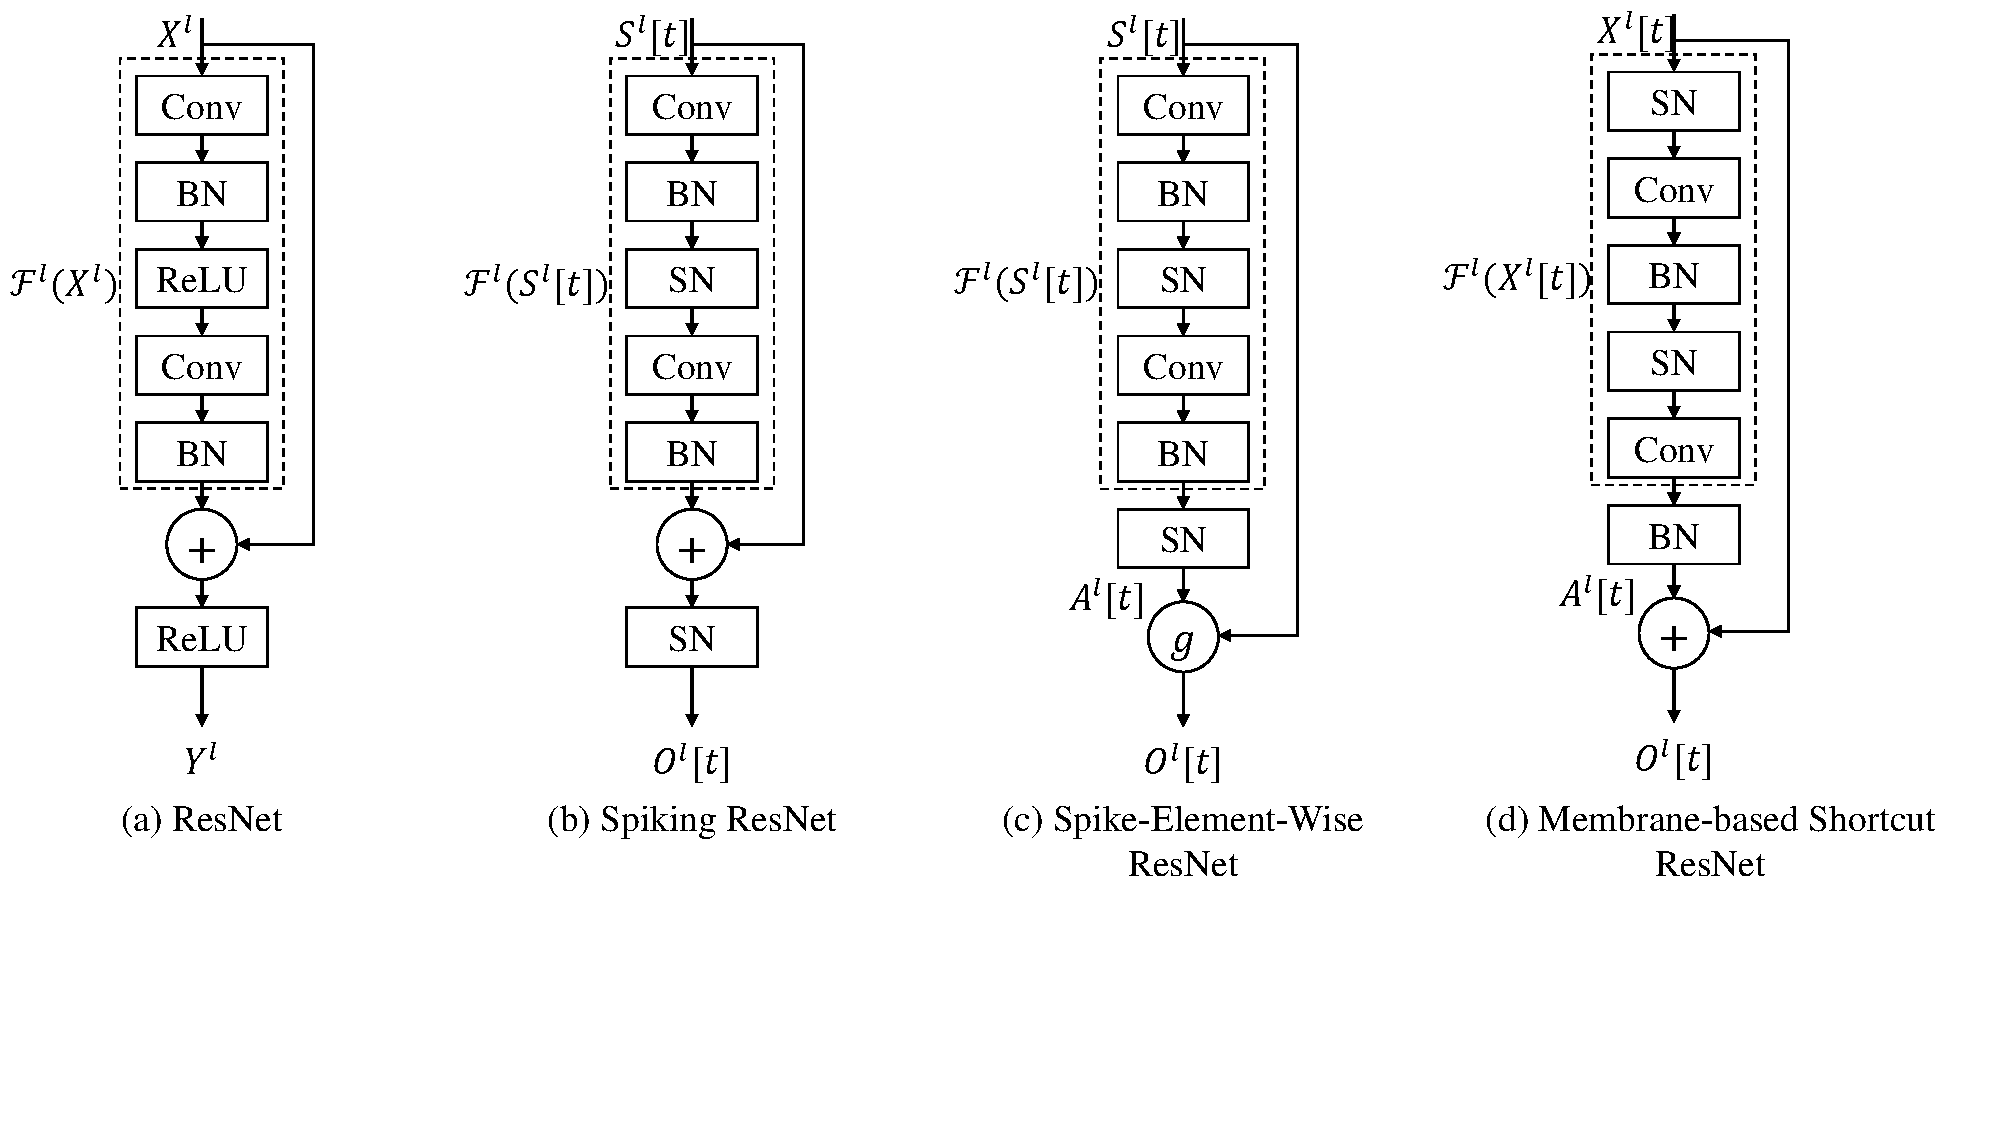
\includegraphics[width=1.\textwidth,trim=0 110 0 0,clip]{./data/res_block.pdf}}
	{\zihao{5}图X\quad 常见的残差块结构}
	\label{fig: res block}
\end{figure}

在ResNet中添加额外的注意力(Attention)模块能够提升神经网络的全局建模能力,从而有效提升任务性能\upcite{graves2014generatingsequencesrecurrentneural, bahdanau2014neural, vaswani2017attention}.这一做法在Spiking ResNet中同样有效.Yao等\upcite{Yao_2021_ICCV}提出了时域注意力(Temporal-wise Attention)机制,将输入在宽、高和通道维度上进行平均后,送入由2层多层感知机(Multilayer Perceptron, MLP)组成的小网络处理,并输出注意力分数,然后与不同时刻输入再进行点乘.这个额外插入的2层MLP网络就是注意力模块,起到辅助提取全局信息的作用.通过设计更高效的注意力模块\upcite{Yao_2023_ICCV,yao2023sparser,xu2023enhancing},或者将注意力机制应用于时间、空间、通道等多个维度\upcite{10032591,zhu2022tcja},SNN在各种任务中的性能能得到显著提升.值得一提的是,与注意力ANN相比,受益于事件驱动计算特性,在SNN中增加额外的注意力模块通常会使得整个网络的能耗进一步降低.Yao等的一系列工作\upcite{yao2023sparser,10032591,Yao_2023_ICCV,Yao2024}对这一现象进行了深入分析.Spiking ResNet包含了循环和卷积两种基本操作,这可以提升参数在时间和空间上的利用效率,但也使得SNN具有“时空不变性\upcite{huang2022tada}”,从而导致较差的全局建模能力\upcite{wang2018non}.与此同时,Spiking ResNet的时空不变性还会引入大量的噪声冗余特征\upcite{Yao_2023_ICCV}.注意力模块能够有效抑制SNN中的噪声脉冲,且优化正常特征,因此能够在带来性能提升的同时显著降低能耗.注意力SNN的功能在边缘计算芯片上也得到了验证\upcite{Yao2024,kim2023c,chang202373}.特别是,将注意力SNN部署到时识科技(SynSense)的异步神经形态感算一体Speck芯片\upcite{Yao2024}后,实测数据显示,在DVS128 Gesture数据集上,注意力机制能带来9\%的性能提升,同时平均功耗由9.5mW降低至3.8mW.


\begin{figure}[H]
	\centerline{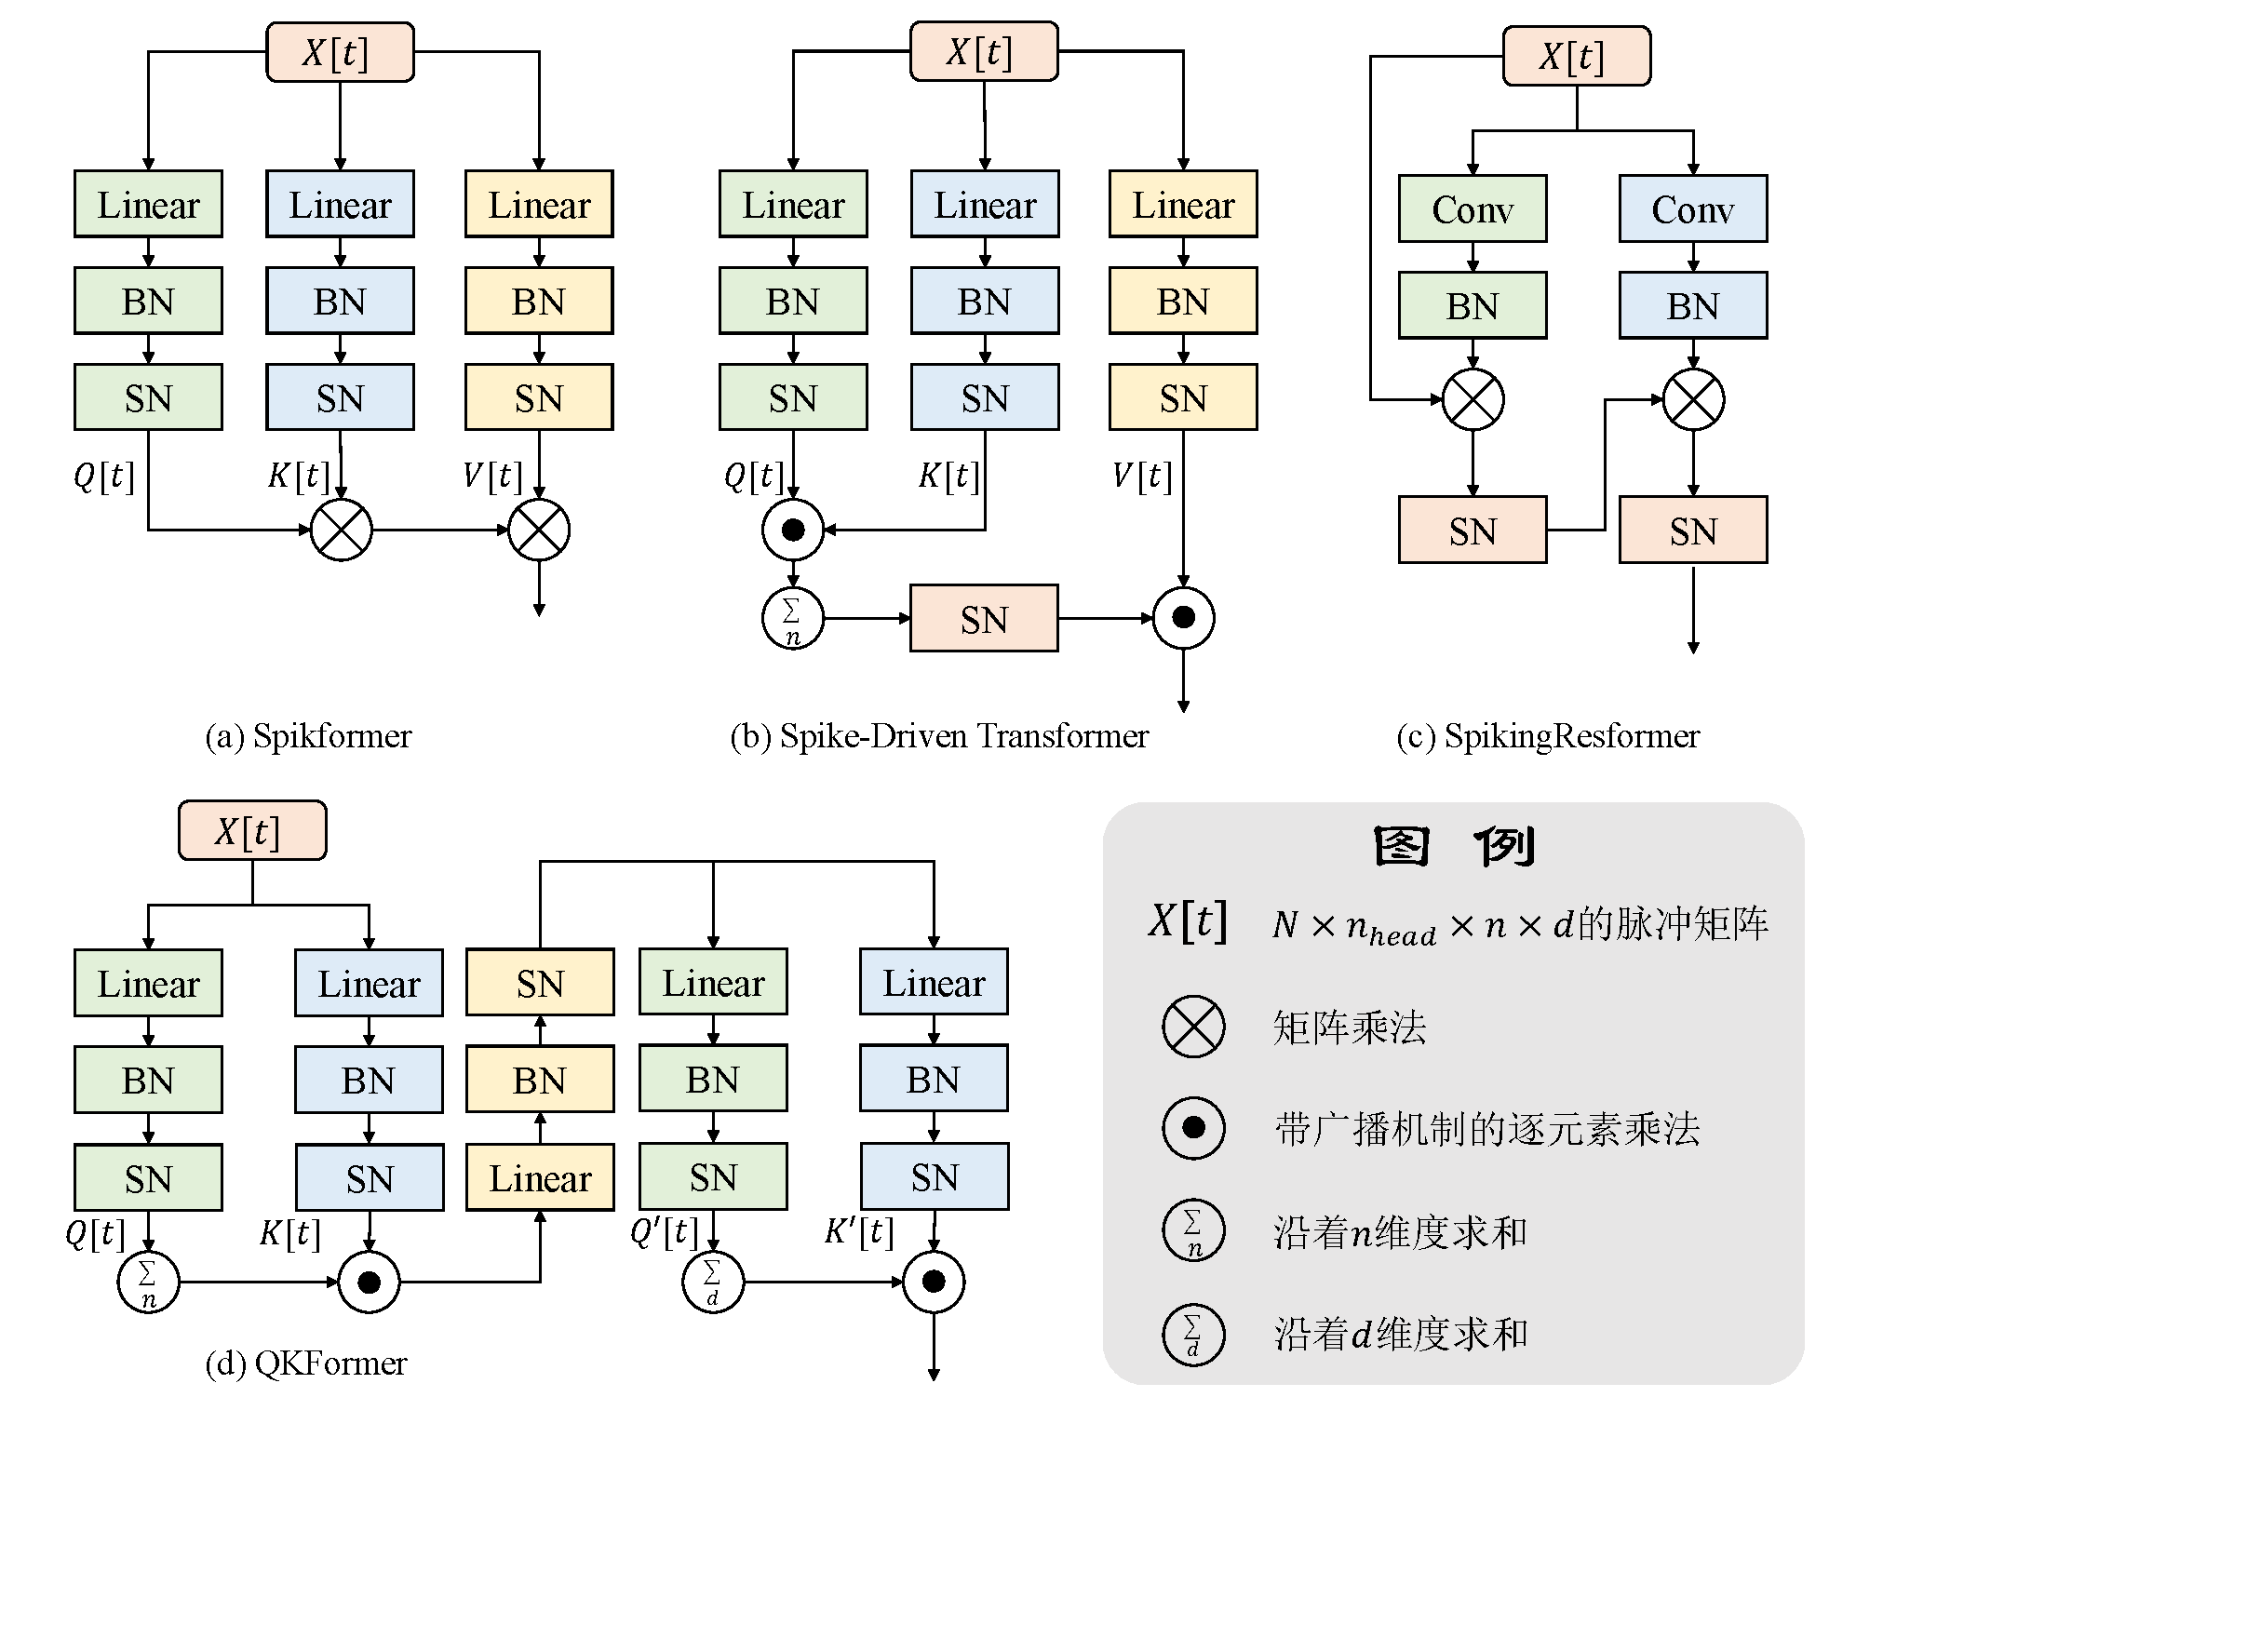
\includegraphics[width=0.95\textwidth]{./data/attention.pdf}}
	{\zihao{5}图X\quad 深度SNN中的自注意力机制}
	\label{fig: self attention}
\end{figure}

以自注意力(Self Attention)机制为基础的Transformer\upcite{vaswani2017attention}是另一类典型的深度学习架构,自提出以来便在多个领域刷新了性能指标,成为目前人工智能领域最常用的网络架构之一.如何有效结合Transformer架构的高性能和SNN的低功耗引起了领域内学者的广泛兴趣.较早的Spiking Transformer\upcite{zhang2022spiking,zhang2022spike,han2023complex}的主要设计思路是,将Transformer中的部分人工神经元改为脉冲神经元,并保留诸如自注意力机制,归一化等关键操作来保证任务精度.这些Spiking Transformer架构事实上是ANN与SNN融合的异构设计,难以真正发挥出SNN低功耗的优势.脉冲深度学习领域的研究者们意识到发挥Spiking Transformer潜力的关键是如何设计脉冲自注意力算子,并围绕这一问题进行了大量改进.图\ref{fig: self attention}展示了目前Spiking Transformer中主流的自注意力机制.

Zhou等\upcite{zhou2023spikformer}指出,自注意力使用的浮点矩阵乘法以及Softmax激活涉及的指数运算难以在神经形态芯片上实现.为此,Zhou等\upcite{zhou2023spikformer}提出了Spikformer,使用脉冲自注意力(Spiking Self Attention, SSA)机制,如图\ref{fig: self attention}(a)所示.对于脉冲神经元的输出$Q[t], K[t], V[t] \in \{0, 1\}^{N \times n_{head} \times n \times d}$,其中$N$表示批量大小,$n_{head}$表示注意力头数,$n$表示分块(Patch)的数量,$d$表示嵌入(Embedding)的维度,则SSA按照如下形式计算注意力分数$score$:
\begin{eqnarray}
	score[t] = \text{SN}(Q[t]K[t]^{\mathrm{T}}V[t] \cdot s), 
\end{eqnarray}
其中$s$是缩放因子,$\text{SN}$表示脉冲神经元层.SSA的两个矩阵乘法参与方都至少包含一个脉冲矩阵,而缩放因子则可以被吸收进脉冲神经元层的阈值;相较于原始的注意力,在SSA中Softmax激活被去掉了,可以根据$n$和$d$来选择先计算$Q[t]K[t]^{\mathrm{T}}$或$K[t]^{\mathrm{T}}V[t]$以降低复杂度至$\text{min}(\mathcal{O}(n^{2}d), \mathcal{O}(nd^{2}))$.

Yao等\upcite{NEURIPS2023_ca0f5358}进一步提出了脉冲驱动Transformer架构,其核心是脉冲驱动自注意力(Spike-Driven Self Attention, SDSA)机制,如图\ref{fig: self attention}(b)所示,其延续了SSA不使用Softmax激活的设计,但使用逐元素乘法替代矩阵乘法,同时去除了自注意力机制中的归一化操作:
\begin{eqnarray}
	score[t] = \text{SN}\Big(\sum_{n}(Q[t]K[t])\Big) \cdot V[t], 
\end{eqnarray}
其中$\sum_{n}$表示沿着分块(Patch)的维度求和.需要注意的是,$\text{SN}(...) \in \{0, 1\}^{N \times n_{head} \times d}$而$V[t]\in \{0, 1\}^{N \times n_{head} \times n \times d}$,两者的逐元素乘法使用了广播(Broadcast)机制.SDSA算子的计算复杂度降低至$\mathcal{O}(nd)$,同时完全消除了乘法,从而使得整个脉冲驱动Transformer中仅有稀疏加法.

SpikingResformer\upcite{Shi_2024_CVPR}使用了双脉冲自注意力机制(Dual Spike Self Attention, DSSA),如图\ref{fig: self attention}(c)所示.这种注意力机制使用了双脉冲变换(Dual Spike Transformation, DST)算子来替换Transformer中的浮点矩阵乘法:
\begin{align}
	&{\rm DST}(X, Y; f(\cdot))=Xf(Y)=XYW,\\
	&{\rm DST_T}(X, Y; f(\cdot))=Xf(Y)^{\rm T}=XW^{\rm T}Y^{\rm T},
\end{align}
其中$f(\cdot)$是$Y$上的广义线性变换,可以是无偏置的线性层、卷积层和BN层等.Shi等\upcite{Shi_2024_CVPR}证明了这种算子是脉冲驱动的,并且可以用这种算子替换Transformer中的浮点矩阵乘法.利用DST算子,DSSA按照如下形式计算注意力分数:
\begin{align}
	&{\rm AttnMap}(X[t])={\rm SN}({\rm DST_T}(X[t], X[t];f(\cdot)) \cdot c_1),\\
	&score[t]={\rm SN}({\rm DST}({\rm AttnMap}(X[t]),X[t];f(\cdot)) \cdot c_2),\\
	&f(X[t])={\rm BN}({\rm Conv_p}(X[t])),
\end{align}
其中$c_1, c_2$是缩放因子,${\rm BN}$是批归一化层,${\rm Conv_p}$是卷积核大小和步长为$p$的卷积.

QKFormer\upcite{zhou2024qkformerhierarchicalspikingtransformer}如其名字所暗示,只使用$Q[t], K[t]$,并通过融合不同维度来提取信息,其结构展示在图\ref{fig: self attention}(d).QKFormer首先在token维度使用脉冲神经元输出的脉冲作为掩模来提取特征:
\begin{eqnarray}
	score[t] = K[t] \cdot \text{SN}\Big(\sum_{n}{Q[t]}\Big),
\end{eqnarray}
其中$K[t] \cdot \text{SN}(...)$用到了广播机制.
QKFormer进而使用相同的操作在通道维度提取特征:
\begin{eqnarray}
	score'[t] = K'[t] \cdot \text{SN}\Big(\sum_{d}{Q'[t]}\Big).
\end{eqnarray}
QKFormer只涉及逐维度求和与逐元素乘法,不使用矩阵乘法,注意力机制的复杂度和脉冲驱动的自注意力类似,也低至$\mathcal{O}(nd)$.

当脉冲化的自注意力机制被成功实现后,研究者们不再使用原有的ResNet等卷积架构作为网络骨架,而是使用Transformer类网络架构,但ResNet中分多个阶段(Stage)的设计得到了保留.

Spikformer\upcite{zhou2023spikformer}和Spike-Driven Transformer\upcite{NEURIPS2023_ca0f5358}使用Compact Convolutional Transformer\upcite{hassani2022escapingbigdataparadigm}的网络架构.
SpikingResformer\upcite{Shi_2024_CVPR}使用了3阶段的层级结构以提取不同尺度的特征,并在2层MLP之间插入分组卷积层以提取局部特征.
Spike-driven Transformer V2\upcite{yao2024spikedriven}专门设计了Meta Transformer块,由带残差连接的Token维度的脉冲驱动的自注意力\upcite{NEURIPS2023_ca0f5358}和通道维度的MLP组成;在网络架构层次,前2个阶段使用带残差连接的大感受野的$7\times7$可分离卷积和小感受野的$3\times3$的普通卷积组成的卷积块,而在后2个阶段使用Meta Transformer块.
QKFormer\upcite{zhou2024qkformerhierarchicalspikingtransformer}则是使用类似Swin Transformer\upcite{liu2021swin}的网络结构.

\begin{figure}[H]
	\centerline{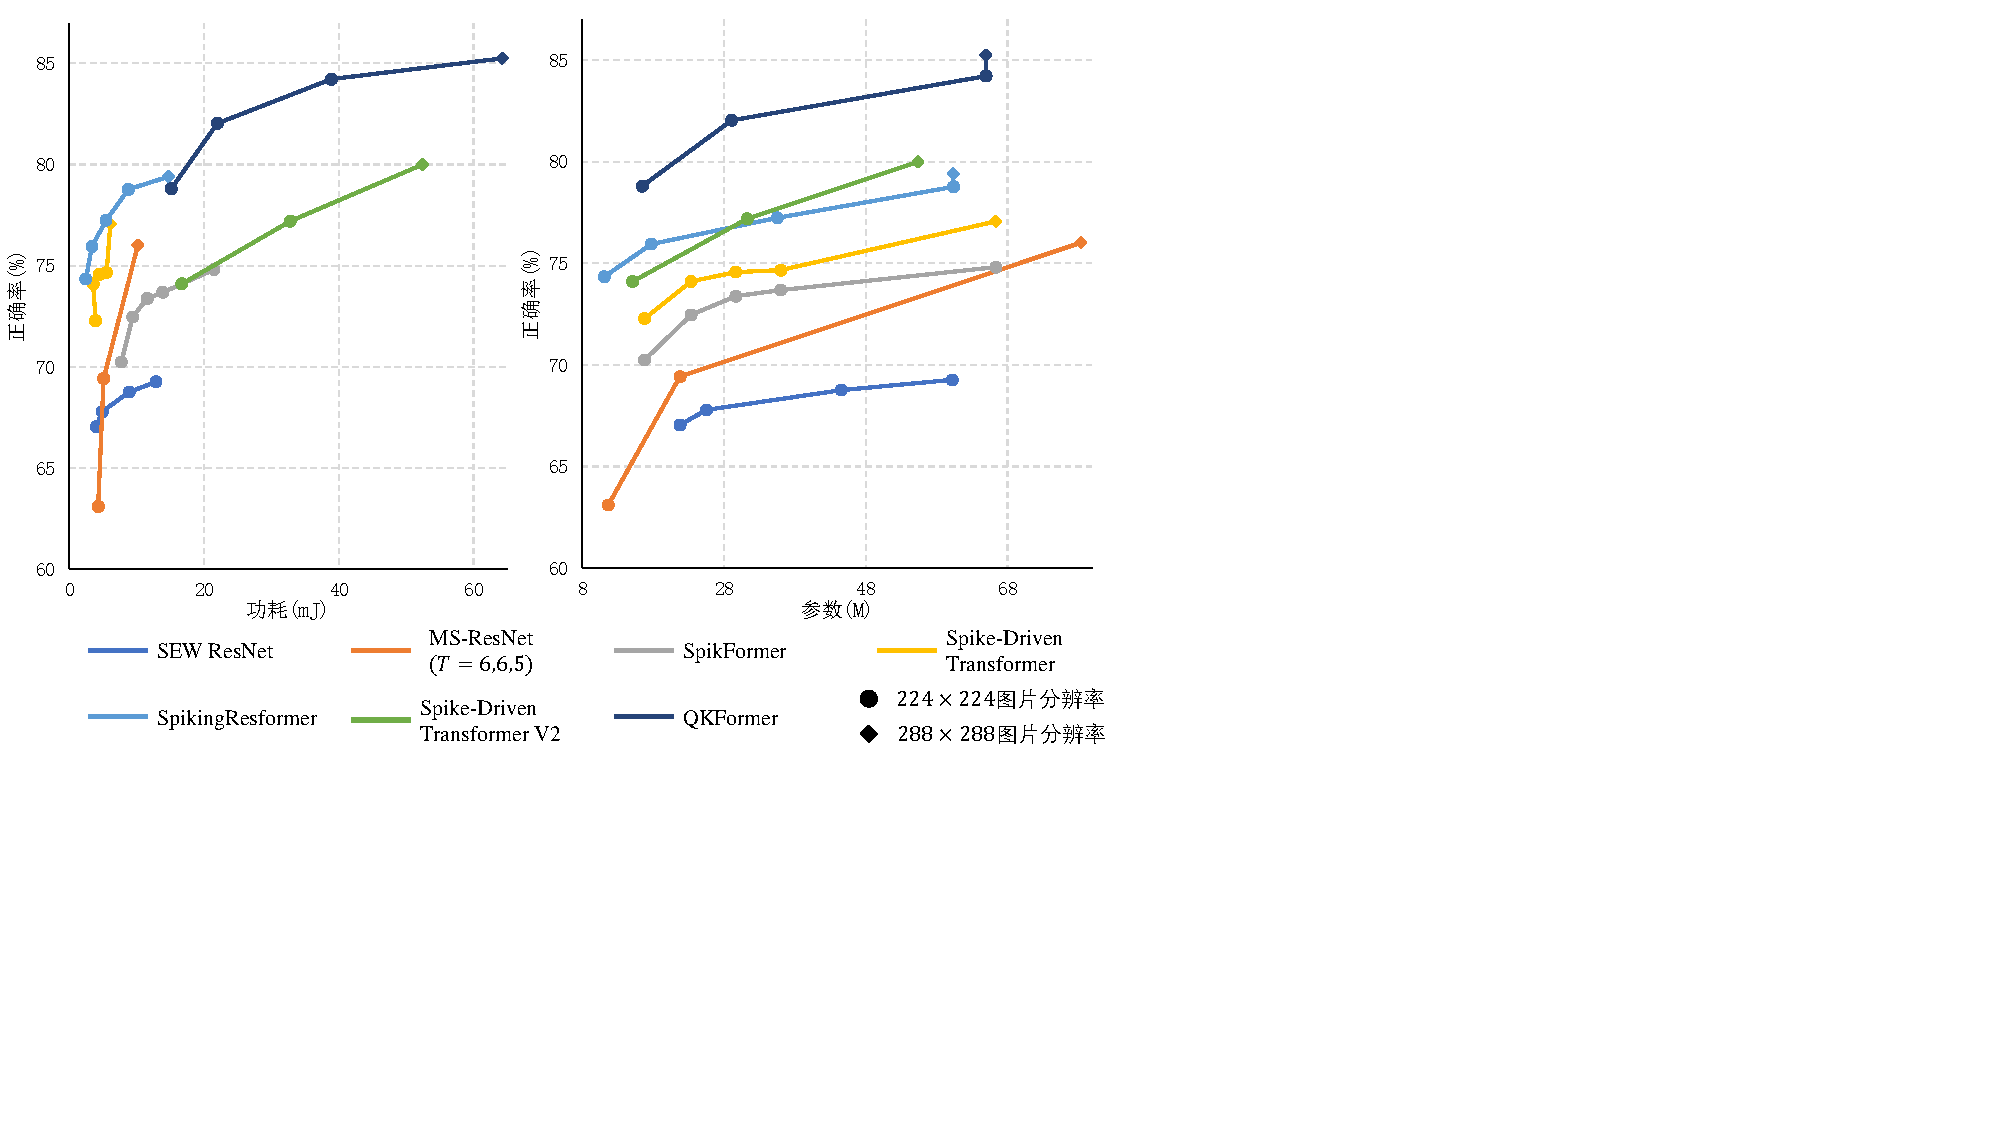
\includegraphics[width=0.9\textwidth,trim=0 180 430 20,clip]{./data/structure_pow_param_acc.pdf}}
	{\zihao{5}图X\quad 常见深度SNN架构在ImageNet数据集的分类正确率、功耗和参数量}
	\label{fig: network structure pow param acc}
\end{figure}

图\ref{fig: network structure pow param acc}对比了常见深度SNN架构在ImageNet数据集的分类正确率、功耗和参数量.除MS-ResNet外,其他网络均使用仿真步数$T=4$;默认使用$224\times224$的图片分辨率进行推理,但也有部分研究者额外汇报了使用$288\times288$图片分辨率推理的结果,在图中以方形点进行了标注.需要说明的是,图\ref{fig: network structure pow param acc}中的功耗皆为理论估算值,其假设SNN在推理时若参与计算的一方是脉冲,则脉冲为0的位置不需要计算,脉冲为1的位置对应的乘法可以使用加法实现;按照每个乘加操作消耗$E_{MAC}=4.6pJ$,每个加法操作则消耗$E_{AC}=0.9pJ$\upcite{6757323};不考虑在内存中读写数据带来的功耗.图\ref{fig: network structure pow param acc}的结果表明,随着残差结构、自注意力机制的引入,深度SNN的性能得到进一步提升,在ImageNet数据集上已经达到85\%的正确率,同时能耗和参数量也不断优化,新的网络架构向着正确率更高且功耗和参数量更低的方向迅猛发展.



除手动设计网络结构外,也有研究者将网络结构搜索技术引入SNN,实现自动化的模型设计.Na等\upcite{na2022autosnn}首次将NAS引入SNN,提出了spike-aware优化方程以限制脉冲数量,通过训练超网和使用遗传算法优化SNN结构;
Kim等\upcite{kim2022neural}提出了新的SNN框架初始化评估指标,通过这一指标避开训练来搜索合适的SNN结构,大幅提升了搜索的速度;
Che等\upcite{che2022differentiable}首次把可微分网络结构搜索方式引入SNN,直接通过训练代理参数来搜索网络结构,提升了训练速度和性能,同时首次将SNN拓展到深度估计等稠密预测领域.

\subsection{正则化方法}% 例如tdbn、tebn
正则化方法已经在神经网络优化过程中大量使用,其中批量标准化(Batch Normalization, BN)\upcite{ioffe2015batch}是SNN中最为广泛使用的方式.相较于层标准化(Layer Normalization)\upcite{ba2016layer}等其他的正则化方法,BN层常用于卷积层之后,并且可以在推理阶段与卷积层融合,无需额外的资源进行实现,因此在SNN中备受青睐.除ANN中已有的正则化方法外,一些专用于SNN的正则化方法也被提出,进一步提升了网络的训练效果.NeuNorm\upcite{neunorm}专用于脉冲卷积层,对于每层神经元,额外记录每个位置$(i, j)$在所有通道的脉冲发放次数之和,并随时间步进行移动平均来持续更新:
\begin{eqnarray}
	O_{norm}[t][i][j] = k_{decay} \cdot O_{norm}[t-1][i][j] + \frac{1 - k_{decay}}{C^{2}} \cdot \sum_{c=0}^{C-1}O[t][c][i][j],
\end{eqnarray}
其中$k_{decay}$是衰减因子,$C$是通道数,$O[t][c][i][j]$是$c$通道位置为$(i, j)$处的神经元在$t$时刻的输出,而$O_{norm}[t][i][j]$则是NeuNorm正则化项,该层传递给下一层的输出会减去该正则化项.NeuNorm对神经元层的输出进行了平滑,可以避免过高或过低的发放率.

在SNN中直接使用普通的BN层可能会造成一些问题,因而研究者们提出了多种BN的变体进行改进,表\ref{tab: bn methods}对目前深度SNN中的BN类方法进行了总结.
普通的BN在SNN中使用时,其训练时会在每个时间步都计算当前$t$时刻输入的均值$\mu[t]$和方差$\sigma[t]$并进行标准化;而在推理时则是利用训练时的统计量来对推理输入标准化.需要注意的是,BN在训练时每次前向传播后都会按照动量的方式来更新均值和方差统计量.记在本次训练前均值和方差统计量分别为$\mu_{k},\sigma_{k}$,其中下标$k$表示统计量更新次数,则经过本次训练后,BN实际上进行了$T$次统计量的动量更新并得到$\mu_{k+T},\sigma_{k+T}$,展示在表\ref{tab: bn methods}中.BN层通常还设置可学习的仿射变换,其权重和偏置项分别是$\beta,\gamma$,由梯度下降更新.

原始的BN这种随着时间步来动量更新统计量的方式可能并不准确,阈值依赖的BN(Threshold-dependent Batch Normalization, TDBN)\upcite{zheng2020going}解决了这一问题,其将输入在时间维度上进行融合,直接计算整个序列的均值和方差,因而处理完一个序列后,BN的统计量只会动量更新一次,而不是按照原始BN的方式更新$T$次.
TDBN还根据后续神经元的阈值对标准化后的输出做相应的线性缩放,以此抵消SNN中特有的阈值给权重的尺度带来的影响.
考虑到SNN中不同时刻的数据分布可能并不相同,因而通过时间批量标准化(Batch Normalization Through Time, BNTT)\upcite{10.3389/fnins.2021.773954}在每个时间步都使用一个独立的BN层,即均值、方差、统计量、仿射变换都是每个时间步一套单独的参数.
时域有效批量标准化(Temporal Effective Batch Normalization, TEBN)\upcite{duan2022temporal}的思想则是介于TDBN和BNTT之间,其统计整个输入序列的均值和方差,但对每个时刻又设置单独的可学习仿射变换.为减少参数量,TEBN中不同时间步的仿射变换是使用类似于广播机制的方式生成的,其权重和偏置项$\gamma$、 $\beta$只有一套,而每个时间步在使用时则是由可学习参数$p[t]$与$\gamma$、 $\beta$相乘来生成$t$时刻的仿射变换参数.
SNN中的正则化层通常被用于卷积层后、神经元前,用于对脉冲神经元的输入电流进行正则化,但也有例外,例如Guo等\upcite{Guo_2023_ICCV_mpbn}对神经元每一步的膜电位也进行批量标准化并取得了性能提升.

\begin{table}[H]
	\centering {\heiti 表X\quad 深度SNN中的批量标准化类方法}
	% \caption{表说明 *表说明采用黑体*}
	\vspace {-2.5mm}
	\begin{center}
\begin{tabular}{cccccc}
	\toprule
	\hline
	正则化方法                      & $t=0$        & $t=1$        & ... & $t=T-1$ &  统计量更新     \\ \hline
	\multirow{2}{*}{BN~\upcite{ioffe2015batch}}   & $\mu[0],\sigma[0]$   & $\mu[1],\sigma[1]$   & &$\mu[T-1],\sigma[T-1]$      & \makecell[c]{$\mu_{k+T} = (1-\rho)^{T}\mu_{k} + \sum_{t=0}^{T-1}(1-\rho)^{T-1-t}\rho\mu[t]$\\$\sigma_{k+T} = (1-\rho)^{T}\sigma_{k} + \sum_{t=0}^{T-1}(1-\rho)^{T-1-t}\rho\sigma[t]$}  \\ \cline{2-6} 
	& \multicolumn{4}{c}{$\gamma, \beta$}              \\ \hline
	\multirow{2}{*}{TDBN~\upcite{zheng2020going}} & \multicolumn{4}{c}{$\mu, \sigma$}  & \makecell[c]{$\mu_{k+1} = (1 - \rho)\mu_{k} + \rho\mu$ \\ $\sigma_{k+1} = (1 - \rho)\sigma_{k} + \rho\sigma$ }           \\ \cline{2-6} 
	& \multicolumn{4}{c}{$\gamma, \beta$}             \\ \hline
	\multirow{2}{*}{BNTT~\upcite{10.3389/fnins.2021.773954}} & $\mu[0],\sigma[0]$   & $\mu[1],\sigma[1]$   &     & $\mu[T-1],\sigma[T-1]$ & \makecell[c]{$\mu_{k+1}[t] = (1 - \rho)\mu_{k}[t] + \rho\mu[t], t=0,1,...,T-1$ \\ $\sigma_{k+1}[t] = (1 - \rho)\sigma_{k}[t] + \rho\sigma[t], t=0,1,...,T-1$ }    \\ \cline{2-6} 
	& $\beta[0], \gamma[0]$ & $\beta[1], \gamma[1]$ &     & $\beta[T-1], \gamma[T-1]$ &  \\ \hline
	\multirow{2}{*}{TEBN~\upcite{duan2022temporal}} & \multicolumn{4}{c}{$\mu, \sigma$}  & \makecell[c]{$\mu_{k+1} = (1 - \rho)\mu_{k} + \rho\mu$ \\ $\sigma_{k+1} = (1 - \rho)\sigma_{k} + \rho\sigma$ }              \\ \cline{2-6} 
	& $\gamma p[0], \beta p[0]$ & $\gamma p[1], \beta p[1]$ &     & $\gamma p[T-1], \beta p[T-1]$ & \\ \hline
	\bottomrule
\end{tabular}
		\label{tab: bn methods}
	\end{center}
\end{table}

正则化方法除使用正则化层外,还包括使用正则化损失和数据增强等.
Guo等\upcite{Guo_2023_ICCV_rmp}将神经元释放脉冲的过程视作信息的量化,将神经元膜电位与输出脉冲的均方误差作为网络损失的一部分,以此减少量化误差;Deng等\upcite{deng2022temporal}使用每个时间步的输出与目标做交叉熵,然后在不同时间步上进行平均,以此替换传统的先平均每个时间步的输出再做交叉熵的损失,对神经形态数据分类等时域任务有较大的性能提升.
数据增强方法通常在训练集样本上施加诸如亮度、尺寸等变换,以提升网络的泛化能力.ANN领域用于静态图片上的数据增强方法已经比较成熟,而Li等\upcite{li2022neuromorphic}则对神经形态数据增强进行了探索,通过对常用的变换进行随机选取和组合并施加于神经形态数据集,提升了SNN的泛化性能.





\subsection{事件驱动学习算法}% 朱耀宇的工作


在SNN的学习方法中,事件驱动方法使用网络发放的脉冲传递梯度信息,因而可以节省反向传播次数进而节省反向传播的能耗.此外,时序梯度只能被脉冲携带,因此事件驱动方法常使用时序梯度.由于只能依赖脉冲传递梯度信息,事件驱动方法较难训练,网络性能表现普遍不佳.

% Jin等提出了HM2-BP\upcite{HM-2BP},在层间的反向传播中累积了神经元在$1~T$时刻的膜电位,梯度反向传播时下一层膜电位到上一层膜电位里膜电位->输出脉冲->膜电位里,本层输出脉冲->本层膜电位的过程使用了代理梯度法进行近似,代理梯度为线性函数.此外,膜电位->权重的过程中推导了脉冲发放时间对膜电位积分值的影响并进行了相应的梯度反向传播.

% \upcite{ST-RSBP}
% Spike-train level backpropagation for training deep recurrent spiking neural networks 前面这俩是对膜电位积分的,感觉不能算事件驱动

在事件驱动学习方法中,梯度在相邻层之间的传播一般从神经元的输出脉冲传递到释放脉冲时的膜电位,再从该膜电位分别向输入脉冲和对应的突触连接权重传递.Zhang等\upcite{zhang2020temporal}在事件驱动学习的基础上,进一步考虑了脉冲响应模型(Spike Response Model, SRM)神经元中重置核导致的多个脉冲之间的相互作用,从而推导出更为细致的反向传播公式.
Zhu等\upcite{zhu2022training}基于SRM神经元,推导出了事件驱动学习方法在含有神经元的网络层反向传播中具有梯度之和不变性:
\begin{align}
	\sum_j \sum_{t_m(s_j^{(l-1)})} \frac{\partial \mathcal{L}}{\partial t_m(s_j^{(l-1)})} = 
	\sum_i \sum_{t_k(s_i^{(l)})} \frac{\partial \mathcal{L}}{\partial t_k(s_i^{(l)})},
\end{align}
其中等式左边是第$l-1$层所有脉冲携带的梯度之和,其中$j$和$t_m(s_j^{(l-1)})$分别对应第$l-1$层的单个神经元和单个脉冲,等式右边是第$l$层所有脉冲携带的梯度之和.
该工作进一步分析了不含神经元的池化层,改进了平均池化层使其满足梯度之和不变性.
在此基础上,Zhu等\upcite{zhu2024exploring}进一步探究了损失函数对时序的事件驱动学习方法的影响.该研究发现,基于频率的损失函数同样适用于时序的事件驱动学习方案,并针对先前损失函数在目标类别输出神经元上梯度之和与脉冲发放数量差异不成正比的问题,提出了改善型计数损失.此外,该工作还将权重归一化中所使用的比例因子的训练转移至阈值,提升了网络的性能.


\subsection{在线学习算法}% 朱耀宇、孟庆晏的工作

在线学习方法为SNN这种需要多个时间步进行学习和推理的模型提供了一种实时更新权重的策略.这种学习方式避免了通过时间反向传播(Back Propagation Through Time, BPTT)需要存储大量中间状态的需求,因此得以节省内存消耗,适用于资源受限或时间步数较多的场景.

Deep Continuous Local Learning (Decolle)\upcite{kaiser2020synaptic}是最早的深度SNN在线学习方法之一,其针对双指数SRM神经元,通过在每层的输出脉冲后引入一个读取层获取局部损失,实现了学习规则在时间和空间上的局部化.
Online Training Through Time (OTTT)\upcite{xiao2022online}对在线学习方法中层内反向传播进行展开并避免了反向传播中的时间步反向依赖,推导出第$l$层的权重$W^{l}$上的梯度为:
\begin{align}
	\frac{\partial \mathcal{L}}{\partial W^l} = \sum_{t=0}^{T-1} \frac{\partial \mathcal{L}}{\partial S^l[t]} \frac{\partial S^l[t]}{\partial U^l[t]} \left( \frac{\partial U^l[t]}{\partial W^l} + \sum_{k < t} \prod_{i=k}^{t-1} \epsilon^l[i] \frac{\partial U^l[k]}{\partial W^l} \right). \label{eq_online_trace}
\end{align}
其中$ \epsilon^l[t] = \frac{\partial U^l[t+1]}{\partial U^l[t]} + \frac{\partial U^l[t+1]}{\partial  S^l[t]} \frac{\partial  S^l[t]}{\partial u^l[t]}$.
随后OTTT对(\ref{eq_online_trace})式进行简化,只保留了$ \epsilon^l[t]$中膜电位衰减的部分,忽略了来自未来时刻的梯度,从而使得梯度计算能够避免BPTT:
\begin{align}
	\frac{\partial \mathcal{L}}{\partial W^l} = \sum_{t=0}^{T-1} \frac{\partial \mathcal{L}}{\partial S^l[t]} \frac{\partial S^l[t]}{\partial U^l[t]} \left( \sum_{k \leq t} \lambda^{t-k} \frac{\partial U^l[k]}{\partial W^l} \right).
\end{align}
此外,该工作还从理论上论证了其梯度与基于脉冲表征的Differentiation on Spike Representation方法\upcite{meng2022training}之间的正相关性.
Spatial Learning Through Time (SLTT)\upcite{meng2023towards}在OTTT的基础上进行了进一步的资源优化.SLTT随机选取了少量时间步进行反向传播,在其余时间步中省去了反向传播过程,提升了存储效率和计算速度.
而Neuronal Dynamics-based Online Training (NDOT)\upcite{jiang2024ndot}在OTTT的基础上对层内的时间依赖性进行了更细致的建模,没有像OTTT一样简化(\ref{eq_online_trace})式,而是将其中的$ \epsilon^l[t]$替换为了描述连续时间内膜电位变化的$e^l[t] = \frac{ U^l[t] - V_{th} S^l[t]}{ U^l[t-1] - V_{th}  S^l[t-1]}$.
Zhu等\upcite{zhu2024online}则考虑在SNN在线学习中加入归一化机制.由于在线学习过程中无法使用未来信息,而直接在每一步进行BN存在协方差漂移问题,该工作提出了包含BN和线性变换的Online Spiking Renormalization (OSR)模块以保证训练和推理时归一化变换参数的一致性,还引入了在线阈值稳定器以稳定时间步之间的神经元发放率.OSR模块训练时的过程可以用以下公式描述:
\begin{align}
	{\hat{I}}[t] =& \frac{ I[t] - \mu[t]}{\sqrt{\sigma^2[t] + \epsilon}}, \label{eq_OSR_1} \\
	{\tilde{I}}[t] =& \gamma \cdot \left( {\hat{I}}[t] \cdot \text{NoGrad}\left( \frac{\sqrt{\sigma^2[t] + \epsilon}}{\sqrt{\hat{\sigma^2} + \epsilon}} \right) + \text{NoGrad} \left( \frac{\mu[t] - \hat{\mu}}{\sqrt{\hat{\sigma^2} + \epsilon}} \right) \right) + \beta, \label{eq_OSR_2}
\end{align}
在第$t$个时间步中,$ I[t]$是未经变换的输入电流,$\mu[t]$和$\sigma^2[t]$分别是$ I[t]$的均值和方差,$\hat{\mu}$、$\hat{\sigma^2}$分别是BN层内记录的均值和方差统计量,$\hat{I}[t]$是BN变换后的值,$\tilde{I}[t]$是二次线性变换之后的值,$\text{NoGrad}(...)$内的运算不参与反向传播.在推理时,OSR的行为则和BN完全一致.

Hu等\upcite{hu2024highperformance}则使用了另外一种思路,通过实验发现常规BPTT训练中只有最后一层的时序信息对训练所得权重影响大,于是在前向传播中关闭了除最后一层外的时序传播过程.
对于保留了前向时序传播的最后一层,该工作使用可逆模块解决了使用$\mathcal{O}(1)$存储空间记录$\mathcal{O}(T)$步信息的问题,其关键是推导出前一时间步膜电位用后一时间步信息来表示的方法.
此外该工作在网络中使用了ConvNeXt块\upcite{liu2022convnet},并将前一时间步的高层信息融合到了当前时间步的低层信息中以提升网络表现.

\subsection{训练加速方法}
相较于ANN,SNN额外增加了时间维度,在不使用在线学习方法、默认使用BPTT方法训练的情况下,网络的训练耗时和内存消耗通常和总时间步$T$成正比,带来了显著高于ANN的训练开销,如何对SNN训练加速成为研究者们日益关心的话题.GPU拥有强大的并行计算能力,是训练SNN的首选设备,目前已有的SNN训练加速方法都基于GPU和SNN的特性进行设计.

稀疏脉冲梯度下降\upcite{perez-nieves2021sparse}在反向传播时,将满足$|H[t]-V_{th}| \ge B_{th}$的神经元视作不活跃的神经元,并将其脉冲释放过程的梯度$\frac{\partial S[t]}{\partial H[t]}$视作0,从而使得本应稠密的反向传播的计算图变得稀疏,然后使用PyTorch中自带的稀疏计算库进行加速.稀疏脉冲梯度下降方法相较于普通的梯度下降方法,在GPU上最高可达150倍的训练反向传播加速和85\%的内存消耗减少,但其只在简单的全连接SNN上进行了实现和验证.
SpikingJelly框架\upcite{doi:10.1126/sciadv.adi1480}提供了更为通用的深度SNN加速方法.SpikingJelly框架首先定义了SNN传播模式的概念,并提出逐步传播和逐层传播这两种计算图的构建方式.在逐层传播模式下,网络中的每层可以同时接收到尺寸为$T\times N \times ...$的整个序列作为输入,其中$T$是序列长度,$N$是批量大小.对于无状态的卷积、全连接等突触层,SpikingJelly框架提供了包装器,将输入的时间和批量维度融合,即将输入尺寸变换到$TN \times ...$,然后再送入无状态层计算,计算得到的结果再重新拆成序列,恢复到尺寸为$T\times N \times ...$的序列.由于时间维度被当作了批量维度,不同时间步的计算也是并行的,速度远快于传统的通过循环实现的逐步计算.对于有状态的神经元等层,SpikingJelly框架使用自定义的CUDA后端,将神经元遍历所有时间步的迭代计算封装到单个CUDA内核,相较于PyTorch实现的神经元在计算时调用多个小CUDA内核,单个大CUDA内核的调度开销更小、计算速度更快,在$T$较大时能有数十倍加速效果.综合使用无状态层和有状态层的加速方法,SpikingJelly框架相较于其他SNN框架实现的SNN仿真方式,最高可达11倍的训练加速效果.
Luke等\upcite{NEURIPS2023_b9f253c2}提出了一种加速脉冲神经元的时间分组仿真方式,在仿真脉冲神经元时,将时间步分组,每组时间步内忽略神经元的重置过程,从而使得膜电位的计算从迭代计算改为直接求解,并将膜电位与阈值比较,输出脉冲,这一思路与PSN\upcite{fang2023parallel}一致;由于前述过程忽略了重置,会导致输出脉冲数量多于有重置的正常神经元仿真方式,该方法进而对输出脉冲进行修正,仅保留每组时间步内的第一个脉冲.该方法相较于正常仿真过程,性能有所降低,但仿真速度大幅度提升.

\section{综合对比实验}
此前尚未有工作将不同类别的方法进行统一的比较,因而本文选取了各类学习算法中的代表性方法,在相同的设置下进行实验,实验类型包括分类任务性能对比和训练加速性能对比.
\subsection{分类任务性能}
本文使用Fang等\upcite{fang2023parallel}的网络结构,测试各类方法分类静态CIFAR10和序列(Sequential) CIFAR10的任务性能,以此检验各类方法的静态数据集分类性能和长期依赖学习能力.CIFAR10分类设置$T=4$,而序列CIFAR10分类的$T=32$与图片宽度一致;统一使用128通道数的卷积层,训练256轮;默认使用SGD优化器,学习率0.1,如果网络不收敛则再额外调整优化器和学习率.参与比较的方法包括ANN辅助训练算法中的Tandem学习方法\upcite{wu2021tandem}和响应与特征蒸馏\upcite{xu2023constructing}、神经元和突触改进算法中的CLIF神经元\upcite{huang2024clif}和PSN家族\upcite{fang2023parallel}、正则化方法中的TEBN\upcite{duan2022temporal}、在线学习算法中的OSR\upcite{zhu2024online}和训练加速算法中的时间分组仿真方式加速的BlockALIF神经元\upcite{NEURIPS2023_b9f253c2}.需要注意的是,本次实验中并没有纳入网络结构改进类方法,因为这些方法已经在复杂的ImageNet数据集上进行了公平的性能比较,结果如图\ref{fig: network structure pow param acc}所示.除CLIF神经元和PSN家族的网络外,ANN辅助训练类算法的网络中使用IF神经元,其它网络均使用LIF神经元.BlockALIF均使用每组2个时间步,因每组1个时间步则与普通神经元无异,没有任何加速效果;每组更多时间步则性能剧烈下降.对于PSN家族的网络,CIFAR10分类任务使用PSN,而序列CIFAR10分类使用$k=4$的Sliding PSN.%没有纳入事件驱动类方法,因为使用的网络结构较深且规模较大,在实验中尚未将该类方法调试到较好性能.

表\ref{tab: cmp acc}展示了各类学习算法中的代表性方法的任务性能.对于序列CIFAR10分类,由于ANN不能直接处理时域任务,故ANN辅助类方法无法使用,在表\ref{tab: cmp acc}中留白.
对于静态的CIFAR10分类,神经动态中不带衰减的IF神经元表现强于LIF神经元,而序列CIFAR10分类则是神经动态更为复杂的LIF神经元性能更好.
Tandem学习方法由于使用不精确的梯度,性能弱于基于替代函数训练的IF神经元.
蒸馏方法相较于原始的使用IF神经元的网络,性能均有一定提升,其中特征蒸馏提升稍高,且均高于Tandem学习方法,表明来自ANN的知识帮助较大.
在静态CIFAR10分类任务上,PSN性能略高于CLIF神经元,均强于IF神经元;而在序列CIFAR10分类任务上,CLIF神经元相较于LIF神经元提升明显,而Sliding PSN性能又大幅度超越CLIF神经元,表明PSN家族通过直接权重连接替换马尔科夫链,极大增强了长期依赖学习能力,而CLIF神经元增加补充电位的神经动态也有利于缓解梯度随时间的衰减.
TEBN在两种任务上都相较于普通网络提升显著,表明使用全部时刻的统计量和逐时刻的仿射变换有效提升了拟合能力.
OSR作为在线学习方法,在CIFAR10分类任务上性能反而强于普通网络,但在序列CIFAR10分类任务上性能大幅度下降,表明静态任务的梯度较易近似,而动态任务的梯度则很难逼近.
BlockALIF性能较差,而且在$T=32$的序列CIFAR10分类任务上性能下降更严重,表明时间上的分组限制了脉冲发放次数,对性能有着很大的负面影响.
\begin{table}[H]
	\centering {\heiti 表X\quad 对比各类代表性方法任务正确率(\%)}
	% \caption{表说明 *表说明采用黑体*}
	\vspace {-2.5mm}
	\begin{center}
		\begin{tabular}{ccccccccccc}
			\toprule
			& IF    & LIF   & Tandem~\upcite{wu2021tandem} & 响应蒸馏~\upcite{xu2023constructing}  & 特征蒸馏~\upcite{xu2023constructing}  & CLIF~\upcite{huang2024clif}  & PSN家族~\upcite{fang2023parallel} & TEBN~\upcite{duan2022temporal}  & OSR~\upcite{zhu2024online} & BlockALIF~\upcite{NEURIPS2023_b9f253c2}  \\ \hline
			CIFAR10            & 93.04 & 92.98 & 89.36  & 93.11 & 93.18 & 93.21 & 93.22 & 93.32 & 93.21   & 90.27     \\
			序列CIFAR10 & 78.31 & 80.5  &       &      &      & 81.55 & 86.31 & 82.60  & 64.09   & 64.81    \\ 
			\bottomrule
		\end{tabular}
		\label{tab: cmp acc}
	\end{center}
\end{table}


\begin{table}[H]
	\centering {\heiti 表X\quad 对比加速方法性能}
	% \caption{表说明 *表说明采用黑体*}
	\vspace {-2.5mm}
	\begin{center}
		\begin{tabular}{c|cccccc|c}
			\hline
			\multicolumn{1}{c|}{\multirow{3}{*}{$T$}} & \multicolumn{6}{c|}{相较于LIF神经元的加速比}                                                                                     & \multirow{3}{*}{LIF耗时(ms)} \\ \cline{2-7}
			\multicolumn{1}{c|}{}                   & \multirow{2}{*}{SpikingJelly~\upcite{doi:10.1126/sciadv.adi1480}} & \multicolumn{1}{c|}{\multirow{2}{*}{PSN~\upcite{fang2023parallel}}} & \multicolumn{4}{c|}{BlockALIF~\upcite{NEURIPS2023_b9f253c2}分组大小}           &                            \\
			\multicolumn{1}{c|}{}                   &                               & \multicolumn{1}{c|}{}                     & 2    & 4    & 8    & \multicolumn{1}{c|}{16} &                            \\ \hline
			2                                       & 1.03                          & 2.20                                      & 0.20 &      &      &                         & 1.44                       \\
			4                                       & 1.48                          & 4.07                                      & 0.17 & 0.38 & 0.38 &                         & 3.02                       \\
			8                                       & 2.72                          & 6.81                                      & 0.15 & 0.29 & 0.29 &                         & 4.79                       \\
			16                                      & 6.19                          & 12.60                                     & 0.22 & 0.29 & 0.29 & 1.29                    & 9.48                       \\
			32                                      & 16.61                         & 17.76                                     & 0.25 & 0.40 & 0.40 & 1.01                    & 17.14                      \\
			64                                      & 14.83                         & 43.75                                     & 0.24 & 0.45 & 0.45 & 0.98                    & 30.60                      \\ \hline
			\hline                 
		\end{tabular}
		\label{tab: cmp speedup}
	\end{center}
\end{table}


\subsection{加速性能测试}
已有的SNN加速的研究集中在神经元层次,故本文选取PyTorch实现的LIF神经元、测试SpikingJelly框架中融合内核实现的LIF神经元\upcite{doi:10.1126/sciadv.adi1480}、并行脉冲神经元PSN\upcite{fang2023parallel}和时间分组仿真方式加速的BlockALIF神经元\upcite{NEURIPS2023_b9f253c2}进行实验,对比加速性能.实验环境为Intel Core i9-10900X CPU,64G内存,Nvidia RTX 2080 Ti GPU;神经元数量为4096;分别测试不同神经元在仿真步数$T=2,4,8,16,32,64$时进行训练(前向传播、反向传播和梯度下降)的耗时.以PyTorch实现的LIF神经元作为速度基准,其他神经元与LIF神经元的速度之比展示在了表\ref{tab: cmp speedup}中.实验结果显示,随着仿真步数的增大,SpikingJelly优势明显,最高可达接近15倍训练加速效果,原因在于$T$较大时PyTorch实现的神经元会调用大量琐碎的CUDA内核,而融合内核后可以大幅度降低琐碎内核的调度开销;PSN加速效果比SpikingJelly更胜一筹,最高可达近44倍加速,展现了并行加速相较于串行计算的巨大优势;BlockALIF则加速效果较差,只在$T$较大且分组大小较大时能略微快于LIF神经元,其他情况则速度更慢,原因可能在于其使用1维卷积实现并行加速,但Fang等\upcite{fang2023parallel}在实现Sliding PSN时也尝试过1维卷积,指出卷积并行度低、速度慢.值得注意的是,Luke等\upcite{NEURIPS2023_b9f253c2}在带有循环连接的SNN上使用BlockALIF神经元,加速效果优秀,可能的原因是循环的连接的计算量较大,而BlockALIF神经元在每个时间组内只调用一次循环连接,并在这次调用中并行处理多个时间步的循环信息,因此相比于传统SNN的在多个时间步中多次循环计算的方法有着较大速度优势.

\section{总结与展望}
本文介绍了脉冲深度学习中基于梯度替代法直接训练的深度脉冲神经网络学习算法研究进展,将已有算法进行分类,并详细介绍和比较.整体来看,现有算法在很大程度上解决了SNN的学习问题,推动SNN向着更高性能、更低功耗的方向不断前进,使得以SNN为计算模型、神经形态硬件为计算设备并构建超低功耗脉冲智能系统成为现实.


\textbf{基础学习算法}是目前梯度替代法训练SNN的基石,但对其研究主要为实验对比,而理论分析较少,需要研究者们重视.
\textbf{ANN辅助训练算法}中基于ANN耦合的算法梯度误差较大,其本质可以认为是使用脉冲在时间上的累计来计算梯度,因而未来的研究方向可以聚焦于设计低误差的脉冲累计表示方法;而基于ANN蒸馏的算法则主要存在计算代价高、超参数数量多且调试困难的缺陷需要改进;两类方法均不能用于时域任务,而通过循环神经网络(Recurrent Neural Network, RNN)或Transformer辅助训练或许能够解决这一问题.
\textbf{神经元和突触改进方法}通常会不可避免地增加模型的复杂度,甚至引入一些难以在现有硬件上实现的操作,例如CLIF神经元\upcite{huang2024clif}中的Sigmoid激活函数涉及硬件上昂贵的指数运算,Sliding PSN\upcite{fang2023parallel}作为$k$阶神经元需要$k$个历史输入的存储消耗,有状态的突触\upcite{SNN-IIR}也需要额外的资源存储和更新状态.因而,未来的研究中应更多的考虑神经形态硬件兼容性和并行加速算法,以增强模型的实用性.
目前的\textbf{网络结构改进方法}已经取得了较大成功,但整体思路仍然延续了ANN的惯性,而生物神经系统中的反馈连接、侧向抑制等特性尚未得到探索,这些特殊的结构可能是实现人脑级别通用人工智能的关键,有待进一步探索.
\textbf{正则化方法}中BN类方法较多,而其他方法较少,考虑到脉冲化的Transformer架构目前性能更高,而其中更倾向于使用LN,故未来的研究可更多聚焦于LN的变体,尤其是原始的LN无法与卷积层合并这一问题扔有待SNN的研究者解决.
\textbf{事件驱动学习算法}适合硬件实现,但目前还难以训练、性能较低,存在很大改进空间;值得注意的是,事件驱动算法理论上更适合基于稀疏计算的实现方式,使用脉冲发放时刻直接表示脉冲,而目前的事件驱动仿真方式仍然使用基于二值张量的方式表示脉冲,存在很大的计算冗余,如何为事件驱动算法设计一套稀疏加速仿真方式,也是值得研究者们重视的话题.
\textbf{在线学习算法}有望解决SNN使用BPTT训练内存消耗量过大的问题,且适合在神经系统硬件上进行实时学习.该类方法目前在静态数据集上表现优秀,但对时域任务还不能很好的处理,需要引起研究者们关注.
\textbf{训练加速方法}中SpikingJelly\upcite{doi:10.1126/sciadv.adi1480}框架加速效果较好且通用性最强,但其加速思路更类似于加速RNN,没有充分利用脉冲的二值量化、稀疏激活特性;稀疏脉冲梯度下降\upcite{perez-nieves2021sparse}则一定程度上利用了SNN的稀疏特性,但其受限于工程难度,只在MLP上进行了实验,没有在更常用的卷积架构上实现.研究者们如果能够充分利用SNN的特性,通过稀疏计算降低计算量和内存消耗,通过二值脉冲和浮点权重的混合精度运算提升计算速度,则SNN相较于ANN的低功耗优势或许能从仅推理阶段延申到更具实用价值的训练阶段,从而彻底解决现有人工智能训练成本高昂的难题.

%
%基础学习算法、ANN辅助训练算法、神经元和突触改进、网络结构改进、正则化方法、事件驱动学习算法、在线学习算法以及训练加速方法

不可否认的是,作为神经科学和计算科学融合的产物的脉冲深度学习领域,目前灵感多来自于深度学习已有的研究范式,技术路线与量化神经网络、循环神经网络、微型机器学习(TinyML)等领域也存在一定重合.考虑到神经科学在人工智能发展中的历史地位,以及人脑仍是已知最智能的系统这一现实,从大脑的结构功能和运行原理出发,设计脑启发的深度SNN学习算法,或许是推动脉冲深度学习取得下一次重大进展的突破方向.

% 对投稿的基本要求:综述应包括引言、问题与挑战、研究现状分析、未来研究方向、结论等内容。以分析、对比为主,避免堆砌文献或一般性介绍、叙述。

%\vspace {3mm}
%\zihao{5}{
%\noindent \textsf{致\quad 谢}\quad \textit{ *致谢内容.* 致谢}}

\vspace {5mm}
\centerline
{\zihao{5}\textsf{参~考~文~献}}
\zihao{5-} \addtolength{\itemsep}{-1em}
\vspace {1.5mm}
\bibliographystyle{gbt7714-numerical}
\bibliography{ref.bib}

\end{multicols}

%\begin{multicols}{1}
%\noindent {\zihao{5}\bf{附录X}.}
%
%{\zihao{5-}\setlength\parindent{2em}
%*\textbf{附录内容}置于此处,字体为小5号宋体。附录内容包括:\textbf{详细的定理证明、公式推导、原始数据}等*}\\\\
%
%\end{multicols}

\newpage
\begin{multicols}{1}
\begin{biography}[./data/weifang.jpg]
	\noindent
	\textbf{Wei Fang} born in 1996, received his B.S. degree from Department of Automation, Tsinghua University, China in 2019 and Ph.D. degree from School of Computer Science, Peking University in 2024. He is currently the Research Assistant Professor in School of Electronic and Computer Engineering, Shenzhen Graduate School, Peking University. His reearch interests include the learning and network structure of Spiking Neural Networks. He has published many articles in journals such as Science Advances/Nature Communications, Neural Networks and conferences such as NeurIPS/ICML/ICLR/ICCV/IJCAI.
\end{biography}
\columnbreak
%\begin{biography}[./data/weifang.jpg]
\zihao{5-}{
\noindent
\textbf{Yonghong Tian} born in 1975, Ph.D., is currently dean of school of electronic and computer engineering, a Boya Distinguished Professor with the Department of Computer Science and Technology, Peking University, China, and is also the deputy director of Artificial Intelligence Research Center, PengCheng Laboratory, Shenzhen, China. His research interests include neuromorphic vision, brain-inspired computation and multimedia big data. He has co-authored over 200 technical articles in refereed journals such as Science Advances/Nature Communications/Scientific Data, IEEE TPAMI/TNNLS/TIP/TMM/TCSVT/TKDE/TPDS/TCYB, ACM CSUR/TOIS/TOMM and conferences such as NeurIPS/ICML/ICLR/CVPR/ICCV/ECCV/AAAI/IJCAI.
}
%\end{biography}
\end{multicols}


\begin{multicols}{1}
\zihao{5}
\noindent \textbf{Background}

\zihao{5-}{
\setlength\parindent{2em}
Artificial Neural Networks (ANNs) monopolize the current Artificial Intelligence (AI) systems for their higher performance than other computational models. However, the floating activation and intensive computation of ANNs cause high energy consumption. Spiking Neural Networks(SNNs), the third generation of neural network models, are the potential alternatives of ANNs for up to hundreds of times of power efficiency. Modules in SNNs communicate by asynchronous spikes as the human brain, which introduces sparse activations, event-driven computations, and consequently low power consumption.

However, there is still a huge performance gap between SNNs and ANNs, which restricts the practical values of SNNs. Complex temporal dynamics and non-differentiable firing mechanisms make it challenging to design learning methods for SNNs. Traditional bio-inspired learning methods such as the Hebbian rule and the Spike Timing Dependent Plasticity rule are unsupervised algorithms and can only solve simple learning tasks such as classifying the MNIST dataset. Primitive supervised learning methods including SpikeProp, Tempotron, and ReSuMe are limited to train SNNs with a single layer or single spike. Recently, deep learning methods have been introduced into SNNs and overwhelmed previous algorithms, growing into the booming spiking deep learning research community.

The ANN to SNN conversion and surrogate learning methods are two mainstream methods in spiking deep learning. The former is based on rate coding and approximates the activations in ANNs by firing rates in SNNs. However, it requires the SNNs to run many time steps and causes high energy consumption and long latency. It cannot solve temporal tasks because the time dimension is already occupied to represent rates. On the contrary, the surrogate learning methods are more flexible. It re-defines the gradient of the discrete Heaviside function used in spike generation by that of a smooth surrogate function and then is capable of training SNNs directly. It is not based on rate coding and can fully utilize neural dynamics to process temporal tasks such as classifying the neuromorphic data. It is not restricted to rate coding and requires much fewer time steps than the conversion methods.

This survey reviews the latest research advancements of the surrogate learning methods in spiking deep learning. The basic concepts, components, and benchmarks of SNNs are first introduced. Then learning methods are systemically divided into different categories and illustrated. A comprehensive experiment is conducted to compare these methods fairly. The advantages and shortcomings of each category are then presented. Lastly, the future research directions are discussed.

This work is partially supported by the National Natural Science Foundation of China under contracts No.62425101, No.62332002, No.62027804, and No.62088102.
}

\end{multicols}
\end{document}
